\documentclass[10pt,dvipsnames,enabledeprecatedfontcommands]{scrartcl}
\usepackage{lmodern}
\usepackage{amssymb,amsmath}
\usepackage{ifxetex,ifluatex}
\usepackage{fixltx2e} % provides \textsubscript
\ifnum 0\ifxetex 1\fi\ifluatex 1\fi=0 % if pdftex
  \usepackage[T1]{fontenc}
  \usepackage[utf8]{inputenc}
\else % if luatex or xelatex
  \ifxetex
    \usepackage{mathspec}
  \else
    \usepackage{fontspec}
  \fi
  \defaultfontfeatures{Ligatures=TeX,Scale=MatchLowercase}
\fi
% use upquote if available, for straight quotes in verbatim environments
\IfFileExists{upquote.sty}{\usepackage{upquote}}{}
% use microtype if available
\IfFileExists{microtype.sty}{%
\usepackage[]{microtype}
\UseMicrotypeSet[protrusion]{basicmath} % disable protrusion for tt fonts
}{}
\PassOptionsToPackage{hyphens}{url} % url is loaded by hyperref
\usepackage[unicode=true]{hyperref}
\PassOptionsToPackage{usenames,dvipsnames}{color} % color is loaded by hyperref
\hypersetup{
            pdftitle={Taking uncertainty in word embedding bias estimation seriously: a bayesian approach},
            pdfauthor={Alicja Dobrzeniecka and Rafal Urbaniak},
            colorlinks=true,
            linkcolor=Maroon,
            citecolor=Blue,
            urlcolor=blue,
            breaklinks=true}
\urlstyle{same}  % don't use monospace font for urls
\usepackage{color}
\usepackage{fancyvrb}
\newcommand{\VerbBar}{|}
\newcommand{\VERB}{\Verb[commandchars=\\\{\}]}
\DefineVerbatimEnvironment{Highlighting}{Verbatim}{commandchars=\\\{\}}
% Add ',fontsize=\small' for more characters per line
\usepackage{framed}
\definecolor{shadecolor}{RGB}{248,248,248}
\newenvironment{Shaded}{\begin{snugshade}}{\end{snugshade}}
\newcommand{\KeywordTok}[1]{\textcolor[rgb]{0.13,0.29,0.53}{\textbf{#1}}}
\newcommand{\DataTypeTok}[1]{\textcolor[rgb]{0.13,0.29,0.53}{#1}}
\newcommand{\DecValTok}[1]{\textcolor[rgb]{0.00,0.00,0.81}{#1}}
\newcommand{\BaseNTok}[1]{\textcolor[rgb]{0.00,0.00,0.81}{#1}}
\newcommand{\FloatTok}[1]{\textcolor[rgb]{0.00,0.00,0.81}{#1}}
\newcommand{\ConstantTok}[1]{\textcolor[rgb]{0.00,0.00,0.00}{#1}}
\newcommand{\CharTok}[1]{\textcolor[rgb]{0.31,0.60,0.02}{#1}}
\newcommand{\SpecialCharTok}[1]{\textcolor[rgb]{0.00,0.00,0.00}{#1}}
\newcommand{\StringTok}[1]{\textcolor[rgb]{0.31,0.60,0.02}{#1}}
\newcommand{\VerbatimStringTok}[1]{\textcolor[rgb]{0.31,0.60,0.02}{#1}}
\newcommand{\SpecialStringTok}[1]{\textcolor[rgb]{0.31,0.60,0.02}{#1}}
\newcommand{\ImportTok}[1]{#1}
\newcommand{\CommentTok}[1]{\textcolor[rgb]{0.56,0.35,0.01}{\textit{#1}}}
\newcommand{\DocumentationTok}[1]{\textcolor[rgb]{0.56,0.35,0.01}{\textbf{\textit{#1}}}}
\newcommand{\AnnotationTok}[1]{\textcolor[rgb]{0.56,0.35,0.01}{\textbf{\textit{#1}}}}
\newcommand{\CommentVarTok}[1]{\textcolor[rgb]{0.56,0.35,0.01}{\textbf{\textit{#1}}}}
\newcommand{\OtherTok}[1]{\textcolor[rgb]{0.56,0.35,0.01}{#1}}
\newcommand{\FunctionTok}[1]{\textcolor[rgb]{0.00,0.00,0.00}{#1}}
\newcommand{\VariableTok}[1]{\textcolor[rgb]{0.00,0.00,0.00}{#1}}
\newcommand{\ControlFlowTok}[1]{\textcolor[rgb]{0.13,0.29,0.53}{\textbf{#1}}}
\newcommand{\OperatorTok}[1]{\textcolor[rgb]{0.81,0.36,0.00}{\textbf{#1}}}
\newcommand{\BuiltInTok}[1]{#1}
\newcommand{\ExtensionTok}[1]{#1}
\newcommand{\PreprocessorTok}[1]{\textcolor[rgb]{0.56,0.35,0.01}{\textit{#1}}}
\newcommand{\AttributeTok}[1]{\textcolor[rgb]{0.77,0.63,0.00}{#1}}
\newcommand{\RegionMarkerTok}[1]{#1}
\newcommand{\InformationTok}[1]{\textcolor[rgb]{0.56,0.35,0.01}{\textbf{\textit{#1}}}}
\newcommand{\WarningTok}[1]{\textcolor[rgb]{0.56,0.35,0.01}{\textbf{\textit{#1}}}}
\newcommand{\AlertTok}[1]{\textcolor[rgb]{0.94,0.16,0.16}{#1}}
\newcommand{\ErrorTok}[1]{\textcolor[rgb]{0.64,0.00,0.00}{\textbf{#1}}}
\newcommand{\NormalTok}[1]{#1}
\usepackage{longtable,booktabs}
% Fix footnotes in tables (requires footnote package)
\IfFileExists{footnote.sty}{\usepackage{footnote}\makesavenoteenv{long table}}{}
\usepackage{graphicx,grffile}
\makeatletter
\def\maxwidth{\ifdim\Gin@nat@width>\linewidth\linewidth\else\Gin@nat@width\fi}
\def\maxheight{\ifdim\Gin@nat@height>\textheight\textheight\else\Gin@nat@height\fi}
\makeatother
% Scale images if necessary, so that they will not overflow the page
% margins by default, and it is still possible to overwrite the defaults
% using explicit options in \includegraphics[width, height, ...]{}
\setkeys{Gin}{width=\maxwidth,height=\maxheight,keepaspectratio}
\IfFileExists{parskip.sty}{%
\usepackage{parskip}
}{% else
\setlength{\parindent}{0pt}
\setlength{\parskip}{6pt plus 2pt minus 1pt}
}
\setlength{\emergencystretch}{3em}  % prevent overfull lines
\providecommand{\tightlist}{%
  \setlength{\itemsep}{0pt}\setlength{\parskip}{0pt}}
\setcounter{secnumdepth}{5}
% Redefines (sub)paragraphs to behave more like sections
\ifx\paragraph\undefined\else
\let\oldparagraph\paragraph
\renewcommand{\paragraph}[1]{\oldparagraph{#1}\mbox{}}
\fi
\ifx\subparagraph\undefined\else
\let\oldsubparagraph\subparagraph
\renewcommand{\subparagraph}[1]{\oldsubparagraph{#1}\mbox{}}
\fi

% set default figure placement to htbp
\makeatletter
\def\fps@figure{htbp}
\makeatother

%\documentclass{article}

% %packages
 \usepackage{booktabs}

\usepackage{multirow}

\usepackage{graphicx}
\usepackage{longtable}
\usepackage{ragged2e}
\usepackage{etex}
%\usepackage{yfonts}
\usepackage{marvosym}
\usepackage[notextcomp]{kpfonts}
\usepackage{nicefrac}
\newcommand*{\QED}{\hfill \footnotesize {\sc Q.e.d.}}
\usepackage{floatrow}

\usepackage[textsize=footnotesize]{todonotes}
%\linespread{1.5}


\setlength{\parindent}{10pt}
\setlength{\parskip}{1pt}


%language
\usepackage{times}
\usepackage{t1enc}
%\usepackage[utf8x]{inputenc}
%\usepackage[polish]{babel}
%\usepackage{polski}
\usepackage[utf8]{inputenc}
\usepackage{mathptmx}
\usepackage[scaled=0.88]{helvet}


%AMS
\usepackage{amsfonts}
\usepackage{amssymb}
\usepackage{amsthm}
\usepackage{amsmath}
\usepackage{mathtools}

\usepackage{geometry}
 \geometry{a4paper,left=35mm,top=20mm,}


%environments
\newtheorem{fact}{Fact}



%abbreviations
\newcommand{\ra}{\rangle}
\newcommand{\la}{\langle}
\newcommand{\n}{\neg}
\newcommand{\et}{\wedge}
\newcommand{\jt}{\rightarrow}
\newcommand{\ko}[1]{\forall  #1\,}
\newcommand{\ro}{\leftrightarrow}
\newcommand{\exi}[1]{\exists\, {_{#1}}}
\newcommand{\pr}[1]{\mathsf{P}(#1)}
\newcommand{\cost}{\mathsf{cost}}


\newcommand{\odds}{\mathsf{Odds}}
\newcommand{\ind}{\mathsf{Ind}}
\newcommand{\nf}[2]{\nicefrac{#1\,}{#2}}
\newcommand{\R}[1]{\texttt{#1}}
\newcommand{\prr}[1]{\mbox{$\mathtt{P}_{prior}(#1)$}}
\newcommand{\prp}[1]{\mbox{$\mathtt{P}_{posterior}(#1)$}}



\newtheorem{q}{\color{blue}Question}
\newtheorem{lemma}{Lemma}
\newtheorem{theorem}{Theorem}



%technical intermezzo
%---------------------

\newcommand{\intermezzoa}{
	\begin{minipage}[c]{13cm}
	\begin{center}\rule{10cm}{0.4pt}



	\tiny{\sc Optional Content Starts}
	
	\vspace{-1mm}
	
	\rule{10cm}{0.4pt}\end{center}
	\end{minipage}\nopagebreak 
	}


\newcommand{\intermezzob}{\nopagebreak 
	\begin{minipage}[c]{13cm}
	\begin{center}\rule{10cm}{0.4pt}

	\tiny{\sc Optional Content Ends}
	
	\vspace{-1mm}
	
	\rule{10cm}{0.4pt}\end{center}
	\end{minipage}
	}
%--------------------






















\newtheorem*{reply*}{Reply}
\usepackage{enumitem}
\newcommand{\question}[1]{\begin{enumerate}[resume,leftmargin=0cm,labelsep=0cm,align=left]
\item #1
\end{enumerate}}

\usepackage{float}

% \setbeamertemplate{blocks}[rounded][shadow=true]
% \setbeamertemplate{itemize items}[ball]
% \AtBeginPart{}
% \AtBeginSection{}
% \AtBeginSubsection{}
% \AtBeginSubsubsection{}
% \setlength{\emergencystretch}{0em}
% \setlength{\parskip}{0pt}






\usepackage[authoryear]{natbib}

%\bibliographystyle{apalike}

\title{Taking uncertainty in word embedding bias estimation seriously: a
bayesian approach}
\author{Alicja Dobrzeniecka and Rafal Urbaniak}
\date{}

\begin{document}
\maketitle

\tableofcontents

\section{Cosine-based measures of
bias}\label{cosine-based-measures-of-bias}

Modern Natural Language Processing (NLP) models are used to complete
various tasks such as providing email filters, smart assistants, search
results, language translations, text analytics and so on. All of them
need as an input words represented by means of numbers which is
accomplished with word embeddings. It seems that in the learning process
these models can learn implicit biases that reflect harmful
stereotypical thinking. One of the sources of bias in NLP can be located
in the way the word embeddings are made. There is a considerable amount
of literature available on the topic of bias detection and mitigation in
NLP models.

One of the first measures in the discussion has been developed by
({\textbf{???}}). There, the gender bias of a word \(w\) is understood
as its projection on the gender direction
\(\vec{w} \cdot (\overrightarrow{he} - \overrightarrow{she})\) (the
gender direction is the top principal compontent of ten gender pair
difference vectors). The underlying idea is that no bias is present if
non-explicitly gendered words are in equal distance to both elements in
all explicitly gender pairs. Given the (ideally) gender neutral words
\(N\) and the gender direction \(g\) the direct gender bias is defined
as the average distance of the words in \(N\) from \(g\) (\(c\) is a
parameter determining how strict we want to be):

\begin{align}
\mathsf{directBias_c(N,g)} & = \frac{\sum_{w\in N}\vert \mathsf{cos}(\vec{w},g)\vert^c}{\vert N \vert }
\end{align}

The use of projections has been ciriticized for instance by
({\textbf{???}}), who point out that while gender-direction might be an
indicator of bias, it is only one possible manifestation of it, and
reducing a projection of words might be insufficient. For instance,
``math'' and ``delicate'' might be in equal distance to both explicitly
gendered words while being closer to quite different stereotypical
attribute words. Further, the authors point out that most word pairs
preserve similarity under debiasing meant to minimize projection-based
bias.\footnote{({\textbf{???}}) use also another method which involves
  analogies and their evaluations by human users on Mechanical Turk. It
  is discussed and criticized in ({\textbf{???}}).}

To measure bias in word embeddings, ({\textbf{???}}) proposed the Word
Embedding Association Test (WEAT). The idea is that the measure of
biases between two sets of target words, \(X\) and \(Y\), (we call them
protected words) should be quantified in terms of the cosine similarity
between the protected words and attribute words coming from two sets of
stereotype attribute words, \(A\) and \(B\) (we'll call them
attributes). For instance, \(X\) might be a set of male names, \(Y\) a
set of female names, \(A\) might contain stereotypically male-related
career words, and \(B\) stereotypically female-related family words.
WEAT is a modification of the Implicit Association Test (IAT)
({\textbf{???}}) used in psychology and uses almost the same word sets,
allowing for a \emph{prima facie} sensible comparison with bias in
humans. If the person's attitude towards given pair of concept is to be
interpreted as neutral, there should be no noticeable task completion
time difference, and the final value from the formula should be around
0. Let \(f\) be a similarity measure (usually, cosine similarity). The
association difference for a term \(t\) is:

\begin{align}
s(t,A,B) & = \frac{\sum_{a\in A}f(t,a)}{\vert A\vert} - \frac{\sum_{b\in B}f(t,b)}{\vert B\vert}
\end{align}

\noindent then, the association difference between \(A\) a \(B\) is:

\begin{align}
s(X,Y,A,B) & = \sum_{x\in X} s(x,A,B) -  \sum_{y\in Y} s(y,A,B)
\end{align}

\noindent
\(s(X,Y,A,B)\) is the statistic used in the signifcance test, and the
\(p\)-value obtained by bootstrapping: it is the frequency of
\(s(X_i,Y_i,A,B)>s(X,Y,A,B)\) for all equally sized partitions
\(X_i, Y_i\) of \(X\cup Y\). The effect size is computed by normalizing
the difference in means as follows:

\begin{align}
bias(A,B) & = \frac{
\mu(\{s(x,A,B)\}_{x\in X}) -\mu(\{s(y,A,B)\}_{y\in Y}) 
}{
\sigma(\{s(w,A,B)\}_{w\in X\cup Y})
}
\end{align}

({\textbf{???}}) show that significant biases---thus measured--- similar
to the ones discovered by IAT can be discovered in word embeddings.
({\textbf{???}}) extended the methodology to a multilingual and
cross-lingual setting, arguing that using Euclidean distance instead of
similarity does not make much difference, while the bias effects vary
greatly across embedding models (interestingly, with social media-text
trained embeddings being less biased than those based on Wikipedia).

A similar methodology is employed by ({\textbf{???}}), who employ word
embeddings trained on corpora from different decades to study the shifts
in various biases. For instance, to compute the occupational embeddings
bias for women the authors first compute the average vector of vector
emeddings of words that represent women (e.g. ``she'', ``female''), then
calculate the Euclidean distance between this mean vector and words for
occupations. Then they take the mean of these distances and subtract
from it the analogously obtained mean for the average vector of vector
embeddings of words that represent men. Formally they take the relative
norm distance between \(X\) and \(Y\) to be:

\begin{align}
\textsf{relative norm distance} & = \sum_{v_m\in M} \vert \vert v_m - v_X\vert \vert_2 - \vert v_m - v_Y\vert \vert_2
\end{align}

\noindent where the norm used is Euclidean, and \(v_X\) and \(x_Y\) are
average vectors for sets \(X\) and \(Y\) respectively.

Manzini, Lim, Tsvetkov, \& Black (2019) modify WEAT to a multi-class
setting, introducing Mean Average Cosine similarity as a measure of bias
(in fact, in the paper they report distances rather than similarities).
Let \(T = \{t_1, \dots, t_k\}\) be a class of protected word embeddings,
and let each \(A_j\in A\) be a set of attributes stereotypically
associated with a protected word). Then:

\begin{align}
S(t_i, A_j) & = \frac{1}{\vert A_j\vert}\sum_{a\in A_j}\mathsf{cos}(t,a) \\
MAC(T,A) & = \frac{1}{\vert T \vert \,\vert A\vert}\sum_{t_i \in T }\sum_{A_j \in A} S(t_i,A_j)
\end{align}

That is, for each protected word \$T and each attribute class, they
first take the mean for this protected word and all attributes in a
given attribute class, and then take the mean of thus obtained means for
all the protected words. The t-tests they employ are run on average
cosines used to calculate MAC.

\section{Some methodological
problems}\label{some-methodological-problems}

\textbf{1. Selection of attributes}

The attributes are taken from different sources, there is no principled
justification for their choice. From our analysis it will become clear
that the list is rather uneven.

There is no mention of methodology for deciding on the number of
attributes necessary to decide a hypothesis on the given size of
dataset. There are however some ways to estimate sample sizes needed to
ensure that the results are meaningful if the effect is present. Our
research will show that the numbers used are rather insufficient.

\textbf{2. No attention to distributions and details}

The authors use the mean of mean average cosine similarities to measure
multi-class similarity between protected word and harmful stereotypes.
They average the results until they obtain one final value to represent
the mean cosine distance between protected word from a given class and
the attributes of that class. If one takes closer look at the individual
values that are taken for the calculations it turns out that there is a
bunch of outliers and surprisingly dissimilar words. We approach this
issue by providing the tables and visualizations of individual cosine
distances to make sure that we obtain a proper insight into the data.

\textbf{3. Hiding the impact of uncertainty}

With such a method the uncertainty involved is not really considered
which makes it even more difficult to give reasonable interpretations of
the results. We propose the use of Bayesian method to obtain some
understanding of the influence the uncertainty has on the interpretation
of final results.

\textbf{4. No word class distinction and no control group}

In the original paper, words from all three religions were compared
against all of the stereotypes, which means that there was no
distinction between cases in which the stereotype is associated with a
given religion, as opposed to the situation in which it is associated
with another one. Not all of the stereotypical words have to be
considered as harmful for all of the religions. One should investigate
the religions separately as some of them may have stronger harmful
associations that others. One should also include control groups to have
a way of comparing the stereotypical results with neutral or human-like
words. Later in the text we will explain in details reasons for
introducing control groups. In our analysis, we distinguish between
stereotypes associated with a given group, stereotypes associated with
different groups, and control groups: neutral words and stereotypes-free
human predicates.

\textbf{5. Interpreting the results}

Assuming for a moment that the value of multi-class cosine distance is
correct, one may question the interpretation. Manzini et al. (2019)
summarize the averages of cosine distance per group (gender, race,
religion). For now let us focus now on analyzing the values relating to
religious biases. Here is the relevant fragment of table:

\begin{longtable}[]{@{}ll@{}}
\toprule
Religion Debiasing & MAC\tabularnewline
\midrule
\endhead
Biased & 0.859\tabularnewline
Hard Debiased & 0.934\tabularnewline
Soft Debiased (\(\lambda\) = 0.2) & 0.894\tabularnewline
\bottomrule
\end{longtable}

MAC stand for mean average cosine similarity, although in reality the
the table contains mean distances. What may attract attention is the
fact that the value of cosine distance in ``Biased'' category is already
quite high even before debiasing. High cosine distance indicates low
cosine similarity between values. One could think that average cosine
similarity equal to approximately 0.141 is not significant enough to
consider it as bias. However the authors aim to mitigate ``biases'' in
vectors with such great distance to make it even larger.
Methodologically the question is, on what basis is this small similarity
still considered as a proof of the presence of bias, and whether these
small changes are meaningful. This is in general the problem of scale
and the lack of universal intervals. In contrast, statistical intervals
will help us decide whether a given cosine similarity is high enough to
consider the words to be more similar than if we chose them at random.
We will use highest posterior density intervals, in line with Bayesian
methodology.

\textbf{6. The curse of dimensionality}

In our case, the curse of dimensionality may take place when there is an
increase in the volume of data that results in adding extra dimensions
to the Euclidean space. According to the article
\href{https://analyticsindiamag.com/curse-of-dimensionality-and-what-beginners-should-do-to-overcome-it/}{Curse
of dimensionality at analyticsindiamag.com} as the number of features
increases, it may be harder and harder to obtain useful information from
the data using the available algorithms. One may notice that more data
should contribute to greater amount of information, but more information
also means greater risk of noise and distractions in data. At the same
time, modern solutions are often adapted to smaller dimensions and their
results in higher ones are not intuitive, or may be prone to error.

Using cosine similarity in high dimensions in word embeddings may also
be prone to the curse of dimensionality. According to Venkat (2018)
there are reasons to consider this phenomenon when searching for word
similarities in higher dimensions. An experiment is conducted that aims
at showing how the similarity values and variation change as the number
of dimensions increases. The hypothesis made in the paper states that
two things will happen as the number of dimensions increase. First, the
effort required to measure cosine similarity will be greater, and two,
the similarity between data will blur out and have less variation. The
authors generate random points with increasing number of dimensions
where each dimension of a data point is given a value between 0 and 1.
Then they pick one vector at random from each dimension class and
calculate the cosine similarity between the chosen vector and the rest
of the data. Then they check how the variation of values changes as the
number of dimensions increases. It seems like the more dimensions there
are, the smaller the variance and therefore it is less obvious how to
interpret the resulting cosine similarities. Maybe the scale should be
adjusted to the number of dimensions and variance so that it still gives
us sensible information about data. Yet, according to some articles
cosine similarity in high dimensions is not reliable enough as it may be
the case that choosing words at random may result in similar values as
when picking them consciously.

\begin{figure}
\centering
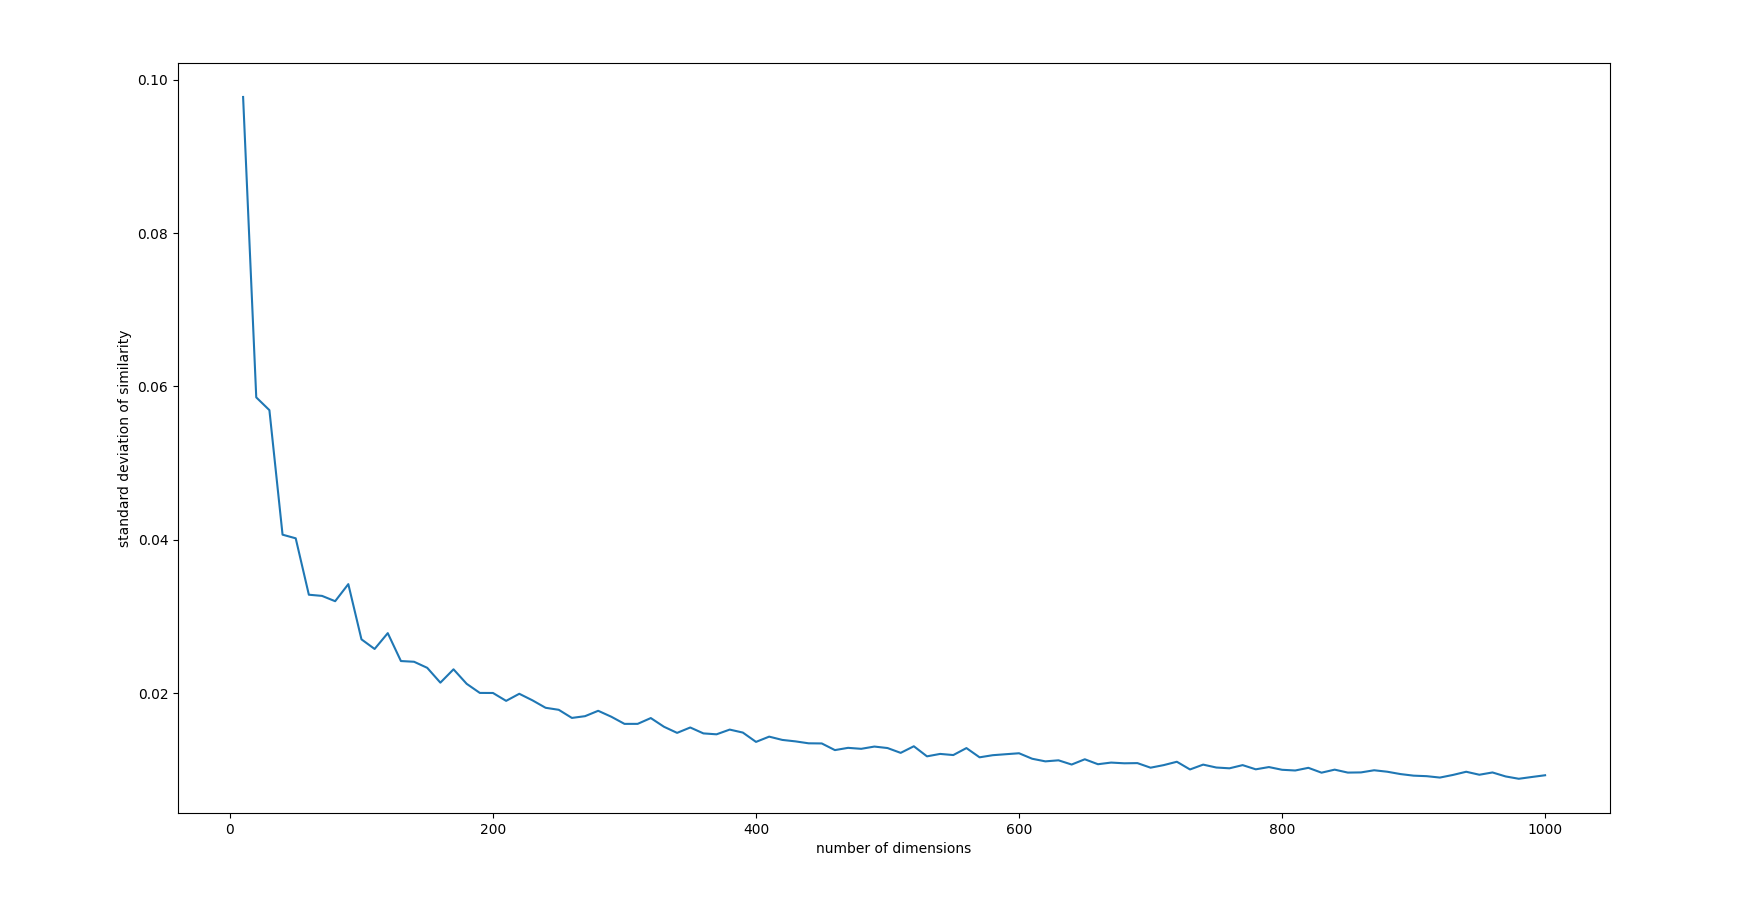
\includegraphics{../images/curseOfDimensionality.png}
\caption{curse of dimensionality, number of dimensions on the x axis,
standard deviation of similarity on the y axis}
\end{figure}

\section{The problem with means of
means}\label{the-problem-with-means-of-means}

The measures described all calculate means of means and their authors
run statistical tests on sets of means. This, however, is problematic
for two related reasons. One, by pre-averaging data we throw away
information about sample sizes. For the former point, think about
proportions: 10 out of 20 and 2 out of 4 give the same mean, but you
would obtain more information by making the former observation rather
than by making the latter. Two, when we pre-average, we remove
variation, and so pre-averaging tend to manufacture false confidence. We
will have more to say about whether this happens in the case of
applications of MAC, for now let's go over a simple example to make the
conceptual point clear.

To illustrate let's employ the formulas used by ({\textbf{???}}) in a
simple example. Conceptually, all such tests come up with rather short
lists of protected words and rather short lists of stereotypical
attributes. Clearly, these are not complete list. So let's treat them as
samples from richer pools of stereotypical predicates and let's take the
uncertainty and variation involved seriously.

Consider a simple situation in which there are two protected classes,
\(X=\{t_1,t_2\}\) and \(Y=\{t_3,t_4\}\) and two five-element attribute
sets \(A\) and \(B\).

First, we play around with a scenario in which all the protected terms
are on average equally unsimilar to both sets (\(\mu =0\)) with standard
deviation of \(.05\). Let's randomly draw similarity scores and plot the
results with group means plotted as vertical lines.

\footnotesize

\begin{Shaded}
\begin{Highlighting}[]
\KeywordTok{set.seed}\NormalTok{(}\DecValTok{123}\NormalTok{)}
\NormalTok{t1 <-}\StringTok{ }\KeywordTok{data.frame}\NormalTok{(}\DataTypeTok{A  =} \KeywordTok{rnorm}\NormalTok{(}\DecValTok{5}\NormalTok{,}\DecValTok{0}\NormalTok{,}\FloatTok{0.05}\NormalTok{), }\DataTypeTok{B =} \KeywordTok{rnorm}\NormalTok{(}\DecValTok{5}\NormalTok{,}\DecValTok{0}\NormalTok{,}\FloatTok{0.05}\NormalTok{))}
\NormalTok{t2 <-}\StringTok{ }\KeywordTok{data.frame}\NormalTok{(}\DataTypeTok{A  =} \KeywordTok{rnorm}\NormalTok{(}\DecValTok{5}\NormalTok{,}\DecValTok{0}\NormalTok{,}\FloatTok{0.05}\NormalTok{), }\DataTypeTok{B =} \KeywordTok{rnorm}\NormalTok{(}\DecValTok{5}\NormalTok{,}\DecValTok{0}\NormalTok{,}\FloatTok{0.05}\NormalTok{))}
\NormalTok{t3 <-}\StringTok{ }\KeywordTok{data.frame}\NormalTok{(}\DataTypeTok{A  =} \KeywordTok{rnorm}\NormalTok{(}\DecValTok{5}\NormalTok{,}\DecValTok{0}\NormalTok{,}\FloatTok{0.05}\NormalTok{), }\DataTypeTok{B =} \KeywordTok{rnorm}\NormalTok{(}\DecValTok{5}\NormalTok{,}\DecValTok{0}\NormalTok{,}\FloatTok{0.05}\NormalTok{))}
\NormalTok{t4 <-}\StringTok{ }\KeywordTok{data.frame}\NormalTok{(}\DataTypeTok{A  =} \KeywordTok{rnorm}\NormalTok{(}\DecValTok{5}\NormalTok{,}\DecValTok{0}\NormalTok{,}\FloatTok{0.05}\NormalTok{), }\DataTypeTok{B =} \KeywordTok{rnorm}\NormalTok{(}\DecValTok{5}\NormalTok{,}\DecValTok{0}\NormalTok{,}\FloatTok{0.05}\NormalTok{))}
\end{Highlighting}
\end{Shaded}

\normalsize

\begin{center}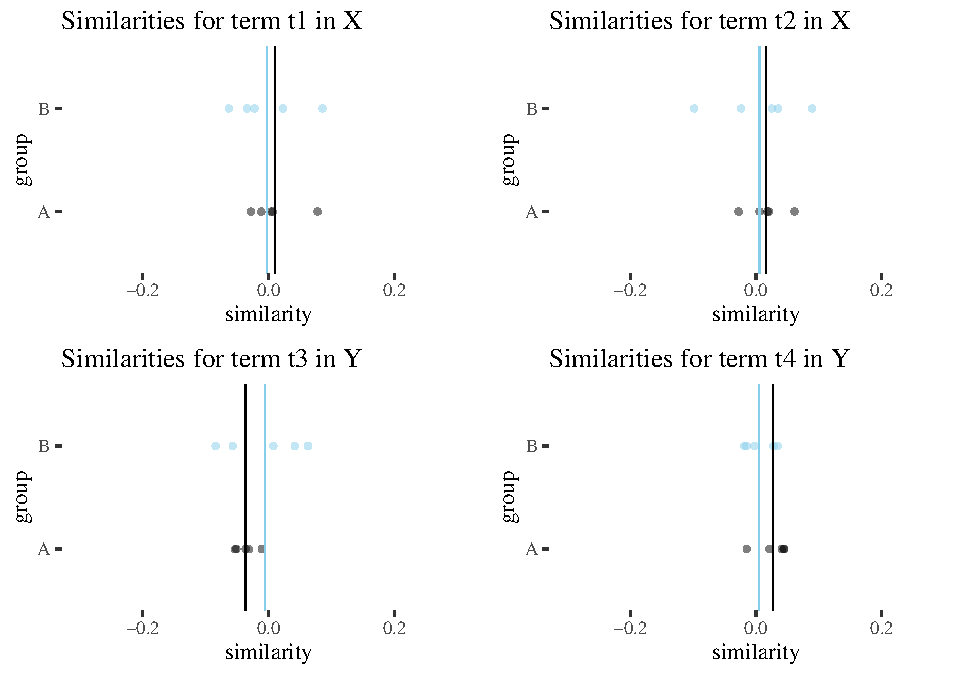
\includegraphics[width=1\linewidth]{paperDraft_files/figure-latex/unnamed-chunk-2-1} \end{center}

\noindent When you look at the datapoints, do you have the impression of
a strong bias here? We wouldn't think so. But now let's run the
calculations from ({\textbf{???}}).

\vspace{1mm} \footnotesize

\begin{Shaded}
\begin{Highlighting}[]
\NormalTok{s <-}\StringTok{ }\ControlFlowTok{function}\NormalTok{ (table)\{ }\KeywordTok{mean}\NormalTok{(table}\OperatorTok{$}\NormalTok{A) }\OperatorTok{-}\StringTok{ }\KeywordTok{mean}\NormalTok{(table}\OperatorTok{$}\NormalTok{B)\}}
\NormalTok{factor <-}\StringTok{ }\KeywordTok{sd}\NormalTok{(}\KeywordTok{c}\NormalTok{(}\KeywordTok{s}\NormalTok{(t1),}\KeywordTok{s}\NormalTok{(t2),}\KeywordTok{s}\NormalTok{(t3),}\KeywordTok{s}\NormalTok{(t4)))}
\NormalTok{numerator <-}\StringTok{  }\KeywordTok{mean}\NormalTok{(}\KeywordTok{s}\NormalTok{(t1),}\KeywordTok{s}\NormalTok{(t2)) }\OperatorTok{-}\StringTok{ }\KeywordTok{mean}\NormalTok{(}\KeywordTok{s}\NormalTok{(t3),}\KeywordTok{s}\NormalTok{(t4))}
\KeywordTok{print}\NormalTok{(}\KeywordTok{list}\NormalTok{(}\DataTypeTok{factor =}\NormalTok{ factor,}\DataTypeTok{numerator =}\NormalTok{ numerator, }\DataTypeTok{bias =}\NormalTok{ numerator }\OperatorTok{/}\StringTok{ }\NormalTok{factor))}
\end{Highlighting}
\end{Shaded}

\begin{verbatim}
## $factor
## [1] 0.02342637
## 
## $numerator
## [1] 0.04275325
## 
## $bias
## [1] 1.825005
\end{verbatim}

\normalsize

\noindent This should make us pause. We know these were points randomly
drawn from distributions where there is no difference in means. Yet, the
calculated effect size is 1.82, whereas the largest effect size reported
by ({\textbf{???}}) is 1.81!

Interestingly, if we repeat the drawing 10000 times, each time
calculating the bias, it turns out that with this variance and sample
size, pretty much anything can happen.

\vspace{1mm} \footnotesize

\begin{Shaded}
\begin{Highlighting}[]
\NormalTok{biasesNull <-}\StringTok{ }\KeywordTok{numeric}\NormalTok{(}\DecValTok{10000}\NormalTok{)}
\ControlFlowTok{for}\NormalTok{(i }\ControlFlowTok{in} \DecValTok{1}\OperatorTok{:}\DecValTok{10000}\NormalTok{)\{}
\NormalTok{t1 <-}\StringTok{ }\KeywordTok{data.frame}\NormalTok{(}\DataTypeTok{A  =} \KeywordTok{rnorm}\NormalTok{(}\DecValTok{5}\NormalTok{,}\DecValTok{0}\NormalTok{,}\FloatTok{0.05}\NormalTok{), }\DataTypeTok{B =} \KeywordTok{rnorm}\NormalTok{(}\DecValTok{5}\NormalTok{,}\DecValTok{0}\NormalTok{,}\FloatTok{0.05}\NormalTok{))}
\NormalTok{t2 <-}\StringTok{ }\KeywordTok{data.frame}\NormalTok{(}\DataTypeTok{A  =} \KeywordTok{rnorm}\NormalTok{(}\DecValTok{5}\NormalTok{,}\DecValTok{0}\NormalTok{,}\FloatTok{0.05}\NormalTok{), }\DataTypeTok{B =} \KeywordTok{rnorm}\NormalTok{(}\DecValTok{5}\NormalTok{,}\DecValTok{0}\NormalTok{,}\FloatTok{0.05}\NormalTok{))}
\NormalTok{t3 <-}\StringTok{ }\KeywordTok{data.frame}\NormalTok{(}\DataTypeTok{A  =} \KeywordTok{rnorm}\NormalTok{(}\DecValTok{5}\NormalTok{,}\DecValTok{0}\NormalTok{,}\FloatTok{0.05}\NormalTok{), }\DataTypeTok{B =} \KeywordTok{rnorm}\NormalTok{(}\DecValTok{5}\NormalTok{,}\DecValTok{0}\NormalTok{,}\FloatTok{0.05}\NormalTok{))}
\NormalTok{t4 <-}\StringTok{ }\KeywordTok{data.frame}\NormalTok{(}\DataTypeTok{A  =} \KeywordTok{rnorm}\NormalTok{(}\DecValTok{5}\NormalTok{,}\DecValTok{0}\NormalTok{,}\FloatTok{0.05}\NormalTok{), }\DataTypeTok{B =} \KeywordTok{rnorm}\NormalTok{(}\DecValTok{5}\NormalTok{,}\DecValTok{0}\NormalTok{,}\FloatTok{0.05}\NormalTok{))}

\NormalTok{factor <-}\StringTok{ }\KeywordTok{sd}\NormalTok{(}\KeywordTok{c}\NormalTok{(}\KeywordTok{s}\NormalTok{(t1),}\KeywordTok{s}\NormalTok{(t2),}\KeywordTok{s}\NormalTok{(t3),}\KeywordTok{s}\NormalTok{(t4)))}
\NormalTok{numerator <-}\StringTok{  }\KeywordTok{mean}\NormalTok{(}\KeywordTok{s}\NormalTok{(t1),}\KeywordTok{s}\NormalTok{(t2)) }\OperatorTok{-}\StringTok{ }\KeywordTok{mean}\NormalTok{(}\KeywordTok{s}\NormalTok{(t3),}\KeywordTok{s}\NormalTok{(t4))}
\NormalTok{biasesNull[i]  <-}\StringTok{ }\NormalTok{numerator }\OperatorTok{/}\StringTok{ }\NormalTok{factor}
\NormalTok{\}}
\KeywordTok{ggplot}\NormalTok{()}\OperatorTok{+}\KeywordTok{geom_histogram}\NormalTok{(}\KeywordTok{aes}\NormalTok{(}\DataTypeTok{x=}\NormalTok{biasesNull, }\DataTypeTok{y =}\NormalTok{ ..density..), }\DataTypeTok{alpha =} \FloatTok{0.6}\NormalTok{, }\DataTypeTok{bins=}\DecValTok{50}\NormalTok{)}\OperatorTok{+}
\StringTok{  }\KeywordTok{theme_tufte}\NormalTok{()}\OperatorTok{+}\KeywordTok{labs}\NormalTok{(}\DataTypeTok{title=}\StringTok{"10k biases for identical means and sd =.05"}\NormalTok{)}\OperatorTok{+}\StringTok{ }\KeywordTok{xlab}\NormalTok{(}\StringTok{"bias"}\NormalTok{)}
\end{Highlighting}
\end{Shaded}

\begin{center}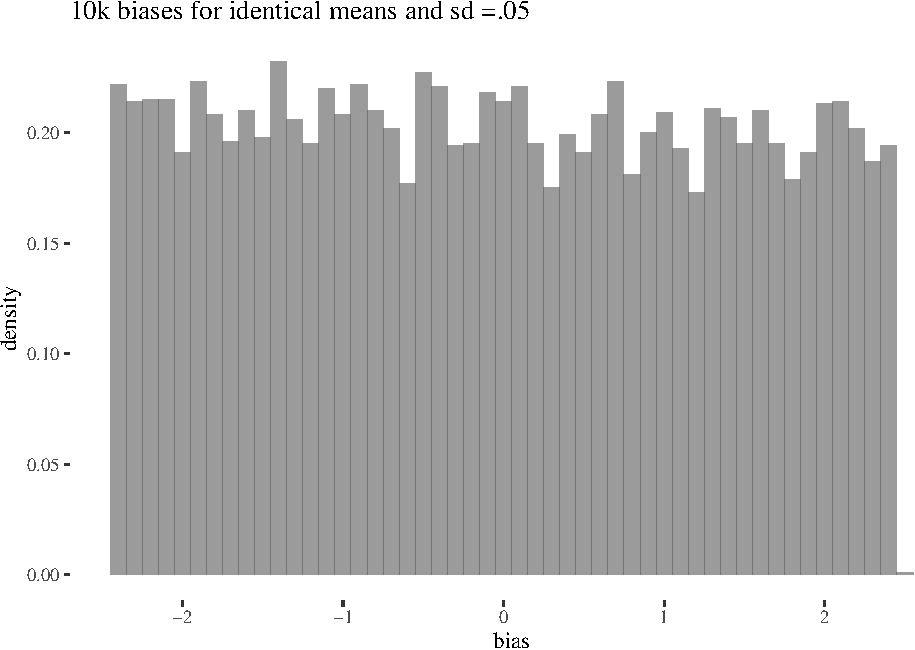
\includegraphics[width=1\linewidth]{paperDraft_files/figure-latex/unnamed-chunk-4-1} \end{center}

\normalsize

Now, let's simulate a situation where the means are identical but the
standard deviation is much smaller, .001.

\footnotesize

\begin{Shaded}
\begin{Highlighting}[]
\KeywordTok{set.seed}\NormalTok{(}\DecValTok{124}\NormalTok{)}
\NormalTok{t1v <-}\StringTok{ }\KeywordTok{data.frame}\NormalTok{(}\DataTypeTok{A  =} \KeywordTok{rnorm}\NormalTok{(}\DecValTok{5}\NormalTok{,}\DecValTok{0}\NormalTok{,}\FloatTok{0.001}\NormalTok{), }\DataTypeTok{B =} \KeywordTok{rnorm}\NormalTok{(}\DecValTok{5}\NormalTok{,}\DecValTok{0}\NormalTok{,}\FloatTok{0.001}\NormalTok{))}
\NormalTok{t2v <-}\StringTok{ }\KeywordTok{data.frame}\NormalTok{(}\DataTypeTok{A  =} \KeywordTok{rnorm}\NormalTok{(}\DecValTok{5}\NormalTok{,}\DecValTok{0}\NormalTok{,}\FloatTok{0.001}\NormalTok{), }\DataTypeTok{B =} \KeywordTok{rnorm}\NormalTok{(}\DecValTok{5}\NormalTok{,}\DecValTok{0}\NormalTok{,}\FloatTok{0.001}\NormalTok{))}
\NormalTok{t3v <-}\StringTok{ }\KeywordTok{data.frame}\NormalTok{(}\DataTypeTok{A  =} \KeywordTok{rnorm}\NormalTok{(}\DecValTok{5}\NormalTok{,}\DecValTok{0}\NormalTok{,}\FloatTok{0.001}\NormalTok{), }\DataTypeTok{B =} \KeywordTok{rnorm}\NormalTok{(}\DecValTok{5}\NormalTok{,}\DecValTok{0}\NormalTok{,}\FloatTok{0.001}\NormalTok{))}
\NormalTok{t4v <-}\StringTok{ }\KeywordTok{data.frame}\NormalTok{(}\DataTypeTok{A  =} \KeywordTok{rnorm}\NormalTok{(}\DecValTok{5}\NormalTok{,}\DecValTok{0}\NormalTok{,}\FloatTok{0.001}\NormalTok{), }\DataTypeTok{B =} \KeywordTok{rnorm}\NormalTok{(}\DecValTok{5}\NormalTok{,}\DecValTok{0}\NormalTok{,}\FloatTok{0.001}\NormalTok{))}
\end{Highlighting}
\end{Shaded}

\normalsize

\begin{center}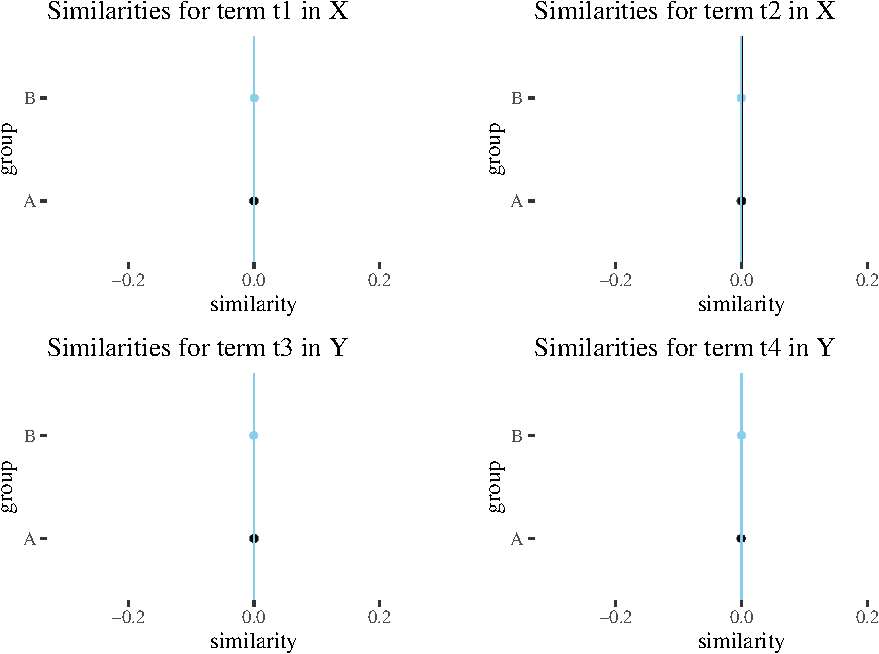
\includegraphics[width=1\linewidth]{paperDraft_files/figure-latex/unnamed-chunk-6-1} \end{center}

\noindent When you look at the datapoints, do you have the impression of
a strong bias here? We wouldn't think so. But now let's run the
calculations from ({\textbf{???}}).

\vspace{1mm} \footnotesize

\begin{Shaded}
\begin{Highlighting}[]
\NormalTok{factorV <-}\StringTok{ }\KeywordTok{sd}\NormalTok{(}\KeywordTok{c}\NormalTok{(}\KeywordTok{s}\NormalTok{(t1v),}\KeywordTok{s}\NormalTok{(t2v),}\KeywordTok{s}\NormalTok{(t3v),}\KeywordTok{s}\NormalTok{(t4v)))}
\NormalTok{numeratorV <-}\StringTok{  }\KeywordTok{mean}\NormalTok{(}\KeywordTok{s}\NormalTok{(t1v),}\KeywordTok{s}\NormalTok{(t2v)) }\OperatorTok{-}\StringTok{ }\KeywordTok{mean}\NormalTok{(}\KeywordTok{s}\NormalTok{(t3v),}\KeywordTok{s}\NormalTok{(t4v))}
\KeywordTok{print}\NormalTok{(}\KeywordTok{list}\NormalTok{(}\DataTypeTok{factor =}\NormalTok{ factorV,}\DataTypeTok{numerator =}\NormalTok{ numeratorV, }\DataTypeTok{bias =}\NormalTok{ numeratorV }\OperatorTok{/}\StringTok{ }\NormalTok{factorV))}
\end{Highlighting}
\end{Shaded}

\begin{verbatim}
## $factor
## [1] 0.0006402666
## 
## $numerator
## [1] -0.001237637
## 
## $bias
## [1] -1.933003
\end{verbatim}

\normalsize

While the numerator and the factors changed a lot, the bias actually
increased. One reason bias increases is that once the standard deviation
goes down, so does the factor used in the calculation of bias.

Again, to see whether this metric would provide us with meaningful
information, let's simulate 10000 drawings.

\vspace{1mm} \footnotesize

\begin{Shaded}
\begin{Highlighting}[]
\KeywordTok{set.seed}\NormalTok{(}\DecValTok{124}\NormalTok{)}

\NormalTok{biasesLowVariance <-}\StringTok{ }\KeywordTok{numeric}\NormalTok{(}\DecValTok{10000}\NormalTok{)}
\ControlFlowTok{for}\NormalTok{(i }\ControlFlowTok{in} \DecValTok{1}\OperatorTok{:}\DecValTok{10000}\NormalTok{)\{}
\NormalTok{t1v <-}\StringTok{ }\KeywordTok{data.frame}\NormalTok{(}\DataTypeTok{A  =} \KeywordTok{rnorm}\NormalTok{(}\DecValTok{5}\NormalTok{,}\DecValTok{0}\NormalTok{,}\FloatTok{0.001}\NormalTok{), }\DataTypeTok{B =} \KeywordTok{rnorm}\NormalTok{(}\DecValTok{5}\NormalTok{,}\DecValTok{0}\NormalTok{,}\FloatTok{0.001}\NormalTok{))}
\NormalTok{t2v <-}\StringTok{ }\KeywordTok{data.frame}\NormalTok{(}\DataTypeTok{A  =} \KeywordTok{rnorm}\NormalTok{(}\DecValTok{5}\NormalTok{,}\DecValTok{0}\NormalTok{,}\FloatTok{0.001}\NormalTok{), }\DataTypeTok{B =} \KeywordTok{rnorm}\NormalTok{(}\DecValTok{5}\NormalTok{,}\DecValTok{0}\NormalTok{,}\FloatTok{0.001}\NormalTok{))}
\NormalTok{t3v <-}\StringTok{ }\KeywordTok{data.frame}\NormalTok{(}\DataTypeTok{A  =} \KeywordTok{rnorm}\NormalTok{(}\DecValTok{5}\NormalTok{,}\DecValTok{0}\NormalTok{,}\FloatTok{0.001}\NormalTok{), }\DataTypeTok{B =} \KeywordTok{rnorm}\NormalTok{(}\DecValTok{5}\NormalTok{,}\DecValTok{0}\NormalTok{,}\FloatTok{0.001}\NormalTok{))}
\NormalTok{t4v <-}\StringTok{ }\KeywordTok{data.frame}\NormalTok{(}\DataTypeTok{A  =} \KeywordTok{rnorm}\NormalTok{(}\DecValTok{5}\NormalTok{,}\DecValTok{0}\NormalTok{,}\FloatTok{0.001}\NormalTok{), }\DataTypeTok{B =} \KeywordTok{rnorm}\NormalTok{(}\DecValTok{5}\NormalTok{,}\DecValTok{0}\NormalTok{,}\FloatTok{0.001}\NormalTok{))}

\NormalTok{factorV <-}\StringTok{ }\KeywordTok{sd}\NormalTok{(}\KeywordTok{c}\NormalTok{(}\KeywordTok{s}\NormalTok{(t1v),}\KeywordTok{s}\NormalTok{(t2v),}\KeywordTok{s}\NormalTok{(t3v),}\KeywordTok{s}\NormalTok{(t4v)))}

\NormalTok{numeratorV <-}\StringTok{  }\KeywordTok{mean}\NormalTok{(}\KeywordTok{s}\NormalTok{(t1v),}\KeywordTok{s}\NormalTok{(t2v)) }\OperatorTok{-}\StringTok{ }\KeywordTok{mean}\NormalTok{(}\KeywordTok{s}\NormalTok{(t3v),}\KeywordTok{s}\NormalTok{(t4v))}

\NormalTok{biasesLowVariance[i] <-}\StringTok{ }\NormalTok{numeratorV }\OperatorTok{/}\StringTok{ }\NormalTok{factorV}
\NormalTok{\}}
\KeywordTok{ggplot}\NormalTok{()}\OperatorTok{+}\KeywordTok{geom_histogram}\NormalTok{(}\KeywordTok{aes}\NormalTok{(}\DataTypeTok{x=}\NormalTok{biasesLowVariance, }\DataTypeTok{y =}\NormalTok{ ..density..), }\DataTypeTok{alpha =} \FloatTok{0.6}\NormalTok{, }\DataTypeTok{bins=}\DecValTok{50}\NormalTok{)}\OperatorTok{+}
\StringTok{  }\KeywordTok{theme_tufte}\NormalTok{()}\OperatorTok{+}\KeywordTok{labs}\NormalTok{(}\DataTypeTok{title=}\StringTok{"10k biases for identical means and sd =.001"}\NormalTok{)}\OperatorTok{+}\StringTok{ }\KeywordTok{xlab}\NormalTok{(}\StringTok{"bias"}\NormalTok{)}
\end{Highlighting}
\end{Shaded}

\begin{center}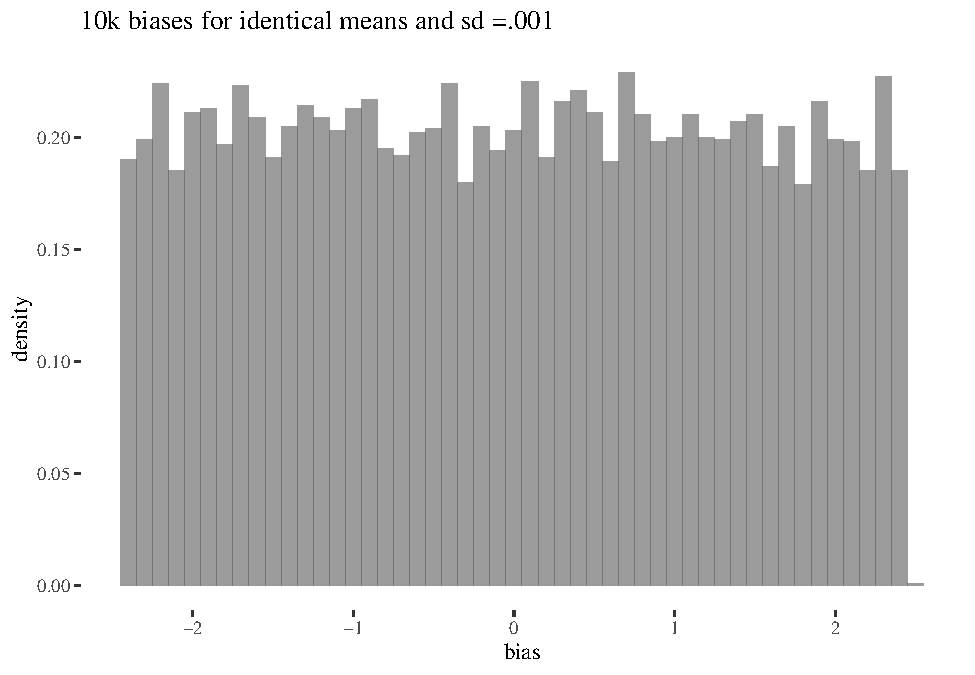
\includegraphics[width=1\linewidth]{paperDraft_files/figure-latex/unnamed-chunk-8-1} \end{center}

\normalsize

Again, not so informative. Now, let's try sampling from distributions
where there in fact is a difference in means. Terms from \(X\) are on
average .1 similar to \(A\) (and still \(0\) to \(B\)), while terms from
\(Y\) are \(.1\) similar to \(B\) (and 0 to \(A\)). The standard
deviation is 0.05 in all the cases. There is a clear difference between
\(X\) and \(Y\) and quick visual inspection should tell us so.

\vspace{1mm} \footnotesize

\begin{Shaded}
\begin{Highlighting}[]
\KeywordTok{set.seed}\NormalTok{(}\DecValTok{766}\NormalTok{)}
\NormalTok{t1d2 <-}\StringTok{ }\KeywordTok{data.frame}\NormalTok{(}\DataTypeTok{A  =} \KeywordTok{rnorm}\NormalTok{(}\DecValTok{5}\NormalTok{,.}\DecValTok{1}\NormalTok{,}\FloatTok{0.05}\NormalTok{), }\DataTypeTok{B =} \KeywordTok{rnorm}\NormalTok{(}\DecValTok{5}\NormalTok{,}\DecValTok{0}\NormalTok{,}\FloatTok{0.05}\NormalTok{))}
\NormalTok{t2d2 <-}\StringTok{ }\KeywordTok{data.frame}\NormalTok{(}\DataTypeTok{A  =} \KeywordTok{rnorm}\NormalTok{(}\DecValTok{5}\NormalTok{,.}\DecValTok{1}\NormalTok{,}\FloatTok{0.05}\NormalTok{), }\DataTypeTok{B =} \KeywordTok{rnorm}\NormalTok{(}\DecValTok{5}\NormalTok{,}\DecValTok{0}\NormalTok{,}\FloatTok{0.05}\NormalTok{))}
\NormalTok{t3d2 <-}\StringTok{ }\KeywordTok{data.frame}\NormalTok{(}\DataTypeTok{A  =} \KeywordTok{rnorm}\NormalTok{(}\DecValTok{5}\NormalTok{,}\DecValTok{0}\NormalTok{,}\FloatTok{0.05}\NormalTok{), }\DataTypeTok{B =} \KeywordTok{rnorm}\NormalTok{(}\DecValTok{5}\NormalTok{,.}\DecValTok{1}\NormalTok{,}\FloatTok{0.05}\NormalTok{))}
\NormalTok{t4d2 <-}\StringTok{ }\KeywordTok{data.frame}\NormalTok{(}\DataTypeTok{A  =} \KeywordTok{rnorm}\NormalTok{(}\DecValTok{5}\NormalTok{,}\DecValTok{0}\NormalTok{,}\FloatTok{0.05}\NormalTok{), }\DataTypeTok{B =} \KeywordTok{rnorm}\NormalTok{(}\DecValTok{5}\NormalTok{,.}\DecValTok{1}\NormalTok{,}\FloatTok{0.05}\NormalTok{))}
\end{Highlighting}
\end{Shaded}

\normalsize

\vspace{1mm} \footnotesize

\begin{center}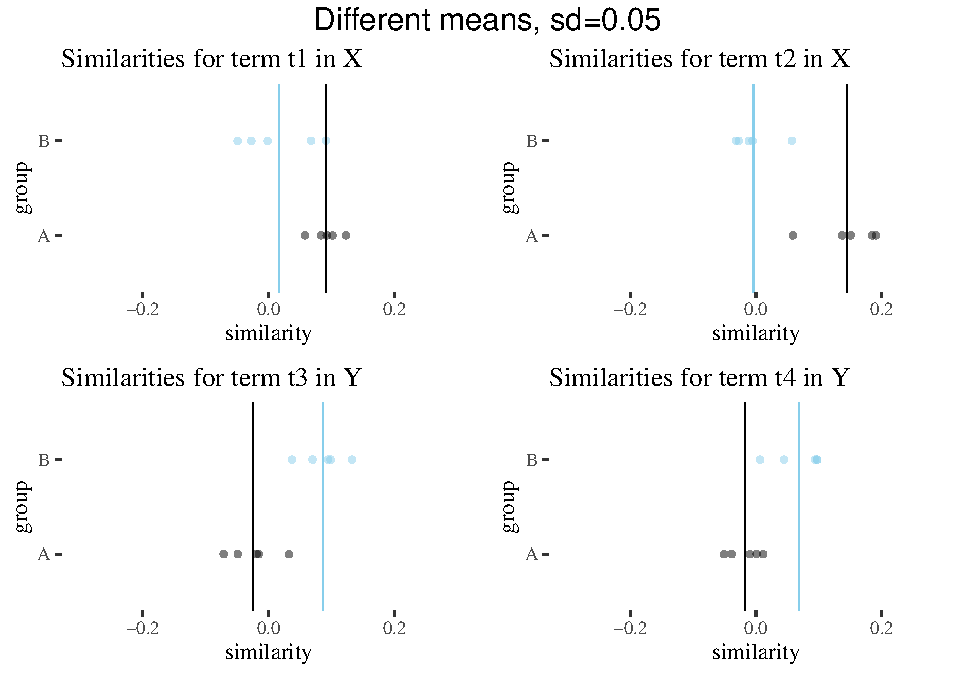
\includegraphics[width=1\linewidth]{paperDraft_files/figure-latex/unnamed-chunk-10-1} \end{center}

\normalsize

\noindent  Is this clear difference mirrored in the calculations?

\footnotesize

\begin{Shaded}
\begin{Highlighting}[]
\NormalTok{factorD2 <-}\StringTok{ }\KeywordTok{sd}\NormalTok{(}\KeywordTok{c}\NormalTok{(}\KeywordTok{s}\NormalTok{(t1d2),}\KeywordTok{s}\NormalTok{(t2d2),}\KeywordTok{s}\NormalTok{(t3d2),}\KeywordTok{s}\NormalTok{(t4d2)))}
\NormalTok{numeratorD2 <-}\StringTok{  }\KeywordTok{mean}\NormalTok{(}\KeywordTok{s}\NormalTok{(t1d2),}\KeywordTok{s}\NormalTok{(t2d2)) }\OperatorTok{-}\StringTok{ }\KeywordTok{mean}\NormalTok{(}\KeywordTok{s}\NormalTok{(t3d2),}\KeywordTok{s}\NormalTok{(t4d2))}
\NormalTok{biasD2 <-}\StringTok{ }\NormalTok{numeratorD2 }\OperatorTok{/}\StringTok{ }\NormalTok{factorD2}
\NormalTok{biasD2}
\end{Highlighting}
\end{Shaded}

\begin{verbatim}
## [1] 1.490014
\end{verbatim}

\normalsize 

\noindent The absolute value of the effect size is smaller than in the
null case with the same standard deviation. Let's simulate 10000
drawings:

\vspace{1mm} \footnotesize

\begin{Shaded}
\begin{Highlighting}[]
\NormalTok{biasesD2 <-}\StringTok{ }\KeywordTok{numeric}\NormalTok{(}\DecValTok{10000}\NormalTok{)}
\ControlFlowTok{for}\NormalTok{(i }\ControlFlowTok{in} \DecValTok{1}\OperatorTok{:}\DecValTok{10000}\NormalTok{)\{}
\NormalTok{t1d2 <-}\StringTok{ }\KeywordTok{data.frame}\NormalTok{(}\DataTypeTok{A  =} \KeywordTok{rnorm}\NormalTok{(}\DecValTok{5}\NormalTok{,.}\DecValTok{1}\NormalTok{,}\FloatTok{0.05}\NormalTok{), }\DataTypeTok{B =} \KeywordTok{rnorm}\NormalTok{(}\DecValTok{5}\NormalTok{,}\DecValTok{0}\NormalTok{,}\FloatTok{0.05}\NormalTok{))}
\NormalTok{t2d2 <-}\StringTok{ }\KeywordTok{data.frame}\NormalTok{(}\DataTypeTok{A  =} \KeywordTok{rnorm}\NormalTok{(}\DecValTok{5}\NormalTok{,.}\DecValTok{1}\NormalTok{,}\FloatTok{0.05}\NormalTok{), }\DataTypeTok{B =} \KeywordTok{rnorm}\NormalTok{(}\DecValTok{5}\NormalTok{,}\DecValTok{0}\NormalTok{,}\FloatTok{0.05}\NormalTok{))}
\NormalTok{t3d2 <-}\StringTok{ }\KeywordTok{data.frame}\NormalTok{(}\DataTypeTok{A  =} \KeywordTok{rnorm}\NormalTok{(}\DecValTok{5}\NormalTok{,}\DecValTok{0}\NormalTok{,}\FloatTok{0.05}\NormalTok{), }\DataTypeTok{B =} \KeywordTok{rnorm}\NormalTok{(}\DecValTok{5}\NormalTok{,.}\DecValTok{1}\NormalTok{,}\FloatTok{0.05}\NormalTok{))}
\NormalTok{t4d2 <-}\StringTok{ }\KeywordTok{data.frame}\NormalTok{(}\DataTypeTok{A  =} \KeywordTok{rnorm}\NormalTok{(}\DecValTok{5}\NormalTok{,}\DecValTok{0}\NormalTok{,}\FloatTok{0.05}\NormalTok{), }\DataTypeTok{B =} \KeywordTok{rnorm}\NormalTok{(}\DecValTok{5}\NormalTok{,.}\DecValTok{1}\NormalTok{,}\FloatTok{0.05}\NormalTok{))}

\NormalTok{factorD2 <-}\StringTok{ }\KeywordTok{sd}\NormalTok{(}\KeywordTok{c}\NormalTok{(}\KeywordTok{s}\NormalTok{(t1d2),}\KeywordTok{s}\NormalTok{(t2d2),}\KeywordTok{s}\NormalTok{(t3d2),}\KeywordTok{s}\NormalTok{(t4d2)))}
\NormalTok{numeratorD2 <-}\StringTok{  }\KeywordTok{mean}\NormalTok{(}\KeywordTok{s}\NormalTok{(t1d2),}\KeywordTok{s}\NormalTok{(t2d2)) }\OperatorTok{-}\StringTok{ }\KeywordTok{mean}\NormalTok{(}\KeywordTok{s}\NormalTok{(t3d2),}\KeywordTok{s}\NormalTok{(t4d2))}
\NormalTok{biasesD2[i] <-}\StringTok{ }\NormalTok{numeratorD2}\OperatorTok{/}\NormalTok{factorD2}
\NormalTok{\}}

\KeywordTok{ggplot}\NormalTok{()}\OperatorTok{+}\KeywordTok{geom_histogram}\NormalTok{(}\KeywordTok{aes}\NormalTok{(}\DataTypeTok{x=}\NormalTok{biasesD2, }\DataTypeTok{y =}\NormalTok{ ..density..), }\DataTypeTok{alpha =} \FloatTok{0.6}\NormalTok{, }\DataTypeTok{bins=}\DecValTok{50}\NormalTok{)}\OperatorTok{+}
\StringTok{  }\KeywordTok{theme_tufte}\NormalTok{()}\OperatorTok{+}\KeywordTok{labs}\NormalTok{(}\DataTypeTok{title=}\StringTok{"10k biases for different means and sd =.05"}\NormalTok{)}\OperatorTok{+}\StringTok{ }\KeywordTok{xlab}\NormalTok{(}\StringTok{"bias"}\NormalTok{)}
\end{Highlighting}
\end{Shaded}

\begin{center}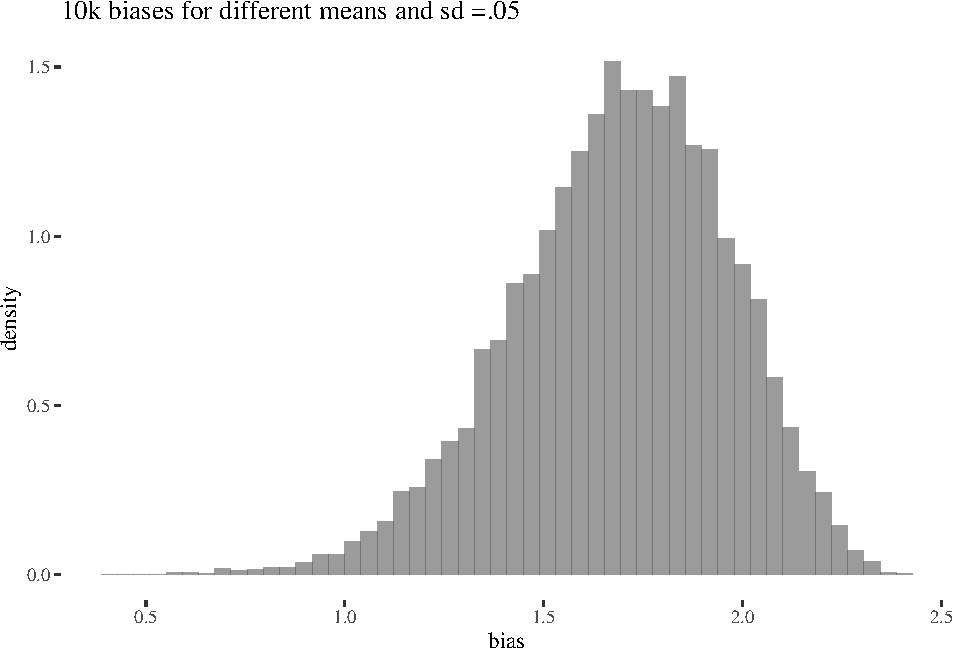
\includegraphics[width=1\linewidth]{paperDraft_files/figure-latex/unnamed-chunk-12-1} \end{center}

\normalsize

\noindent Now suppose we keep the means the same but increase the
standard deviation to .1.

\vspace{1mm} \footnotesize

\begin{Shaded}
\begin{Highlighting}[]
\KeywordTok{set.seed}\NormalTok{(}\DecValTok{766}\NormalTok{)}
\NormalTok{t1d1 <-}\StringTok{ }\KeywordTok{data.frame}\NormalTok{(}\DataTypeTok{A  =} \KeywordTok{rnorm}\NormalTok{(}\DecValTok{5}\NormalTok{,.}\DecValTok{1}\NormalTok{,}\FloatTok{0.1}\NormalTok{), }\DataTypeTok{B =} \KeywordTok{rnorm}\NormalTok{(}\DecValTok{5}\NormalTok{,}\DecValTok{0}\NormalTok{,}\FloatTok{0.1}\NormalTok{))}
\NormalTok{t2d1 <-}\StringTok{ }\KeywordTok{data.frame}\NormalTok{(}\DataTypeTok{A  =} \KeywordTok{rnorm}\NormalTok{(}\DecValTok{5}\NormalTok{,.}\DecValTok{1}\NormalTok{,}\FloatTok{0.1}\NormalTok{), }\DataTypeTok{B =} \KeywordTok{rnorm}\NormalTok{(}\DecValTok{5}\NormalTok{,}\DecValTok{0}\NormalTok{,}\FloatTok{0.1}\NormalTok{))}
\NormalTok{t3d1 <-}\StringTok{ }\KeywordTok{data.frame}\NormalTok{(}\DataTypeTok{A  =} \KeywordTok{rnorm}\NormalTok{(}\DecValTok{5}\NormalTok{,}\DecValTok{0}\NormalTok{,}\FloatTok{0.1}\NormalTok{), }\DataTypeTok{B =} \KeywordTok{rnorm}\NormalTok{(}\DecValTok{5}\NormalTok{,.}\DecValTok{1}\NormalTok{,}\FloatTok{0.1}\NormalTok{))}
\NormalTok{t4d1 <-}\StringTok{ }\KeywordTok{data.frame}\NormalTok{(}\DataTypeTok{A  =} \KeywordTok{rnorm}\NormalTok{(}\DecValTok{5}\NormalTok{,}\DecValTok{0}\NormalTok{,}\FloatTok{0.1}\NormalTok{), }\DataTypeTok{B =} \KeywordTok{rnorm}\NormalTok{(}\DecValTok{5}\NormalTok{,.}\DecValTok{1}\NormalTok{,}\FloatTok{0.1}\NormalTok{))}
\end{Highlighting}
\end{Shaded}

\normalsize

\vspace{1mm} \footnotesize

\begin{center}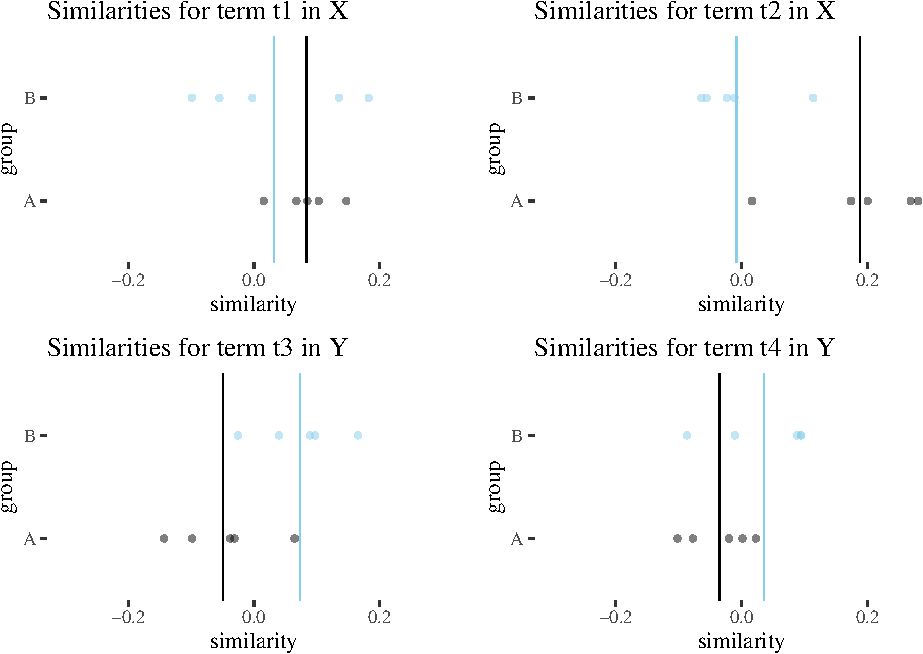
\includegraphics[width=1\linewidth]{paperDraft_files/figure-latex/unnamed-chunk-14-1} \end{center}

\normalsize

\noindent  Is this clear difference mirrored in the calculations?

\footnotesize

\begin{Shaded}
\begin{Highlighting}[]
\NormalTok{factorD1 <-}\StringTok{ }\KeywordTok{sd}\NormalTok{(}\KeywordTok{c}\NormalTok{(}\KeywordTok{s}\NormalTok{(t1d1),}\KeywordTok{s}\NormalTok{(t2d1),}\KeywordTok{s}\NormalTok{(t3d1),}\KeywordTok{s}\NormalTok{(t4d1)))}
\NormalTok{numeratorD1 <-}\StringTok{  }\KeywordTok{mean}\NormalTok{(}\KeywordTok{s}\NormalTok{(t1d1),}\KeywordTok{s}\NormalTok{(t2d1)) }\OperatorTok{-}\StringTok{ }\KeywordTok{mean}\NormalTok{(}\KeywordTok{s}\NormalTok{(t3d1),}\KeywordTok{s}\NormalTok{(t4d1))}
\NormalTok{biasD1 <-}\StringTok{ }\NormalTok{numeratorD1 }\OperatorTok{/}\StringTok{ }\NormalTok{factorD1}
\NormalTok{biasD1}
\end{Highlighting}
\end{Shaded}

\begin{verbatim}
## [1] 1.223023
\end{verbatim}

\normalsize 

\noindent The absolute value of the effect size is smaller than in the
previous case!

\vspace{1mm} \footnotesize

\begin{Shaded}
\begin{Highlighting}[]
\NormalTok{biasesD1 <-}\StringTok{ }\KeywordTok{numeric}\NormalTok{(}\DecValTok{10000}\NormalTok{)}

\ControlFlowTok{for}\NormalTok{(i }\ControlFlowTok{in} \DecValTok{1}\OperatorTok{:}\DecValTok{10000}\NormalTok{)\{}
\NormalTok{t1d1 <-}\StringTok{ }\KeywordTok{data.frame}\NormalTok{(}\DataTypeTok{A  =} \KeywordTok{rnorm}\NormalTok{(}\DecValTok{5}\NormalTok{,.}\DecValTok{1}\NormalTok{,}\FloatTok{0.1}\NormalTok{), }\DataTypeTok{B =} \KeywordTok{rnorm}\NormalTok{(}\DecValTok{5}\NormalTok{,}\DecValTok{0}\NormalTok{,}\FloatTok{0.1}\NormalTok{))}
\NormalTok{t2d1 <-}\StringTok{ }\KeywordTok{data.frame}\NormalTok{(}\DataTypeTok{A  =} \KeywordTok{rnorm}\NormalTok{(}\DecValTok{5}\NormalTok{,.}\DecValTok{1}\NormalTok{,}\FloatTok{0.1}\NormalTok{), }\DataTypeTok{B =} \KeywordTok{rnorm}\NormalTok{(}\DecValTok{5}\NormalTok{,}\DecValTok{0}\NormalTok{,}\FloatTok{0.1}\NormalTok{))}
\NormalTok{t3d1 <-}\StringTok{ }\KeywordTok{data.frame}\NormalTok{(}\DataTypeTok{A  =} \KeywordTok{rnorm}\NormalTok{(}\DecValTok{5}\NormalTok{,}\DecValTok{0}\NormalTok{,}\FloatTok{0.1}\NormalTok{), }\DataTypeTok{B =} \KeywordTok{rnorm}\NormalTok{(}\DecValTok{5}\NormalTok{,.}\DecValTok{1}\NormalTok{,}\FloatTok{0.1}\NormalTok{))}
\NormalTok{t4d1 <-}\StringTok{ }\KeywordTok{data.frame}\NormalTok{(}\DataTypeTok{A  =} \KeywordTok{rnorm}\NormalTok{(}\DecValTok{5}\NormalTok{,}\DecValTok{0}\NormalTok{,}\FloatTok{0.1}\NormalTok{), }\DataTypeTok{B =} \KeywordTok{rnorm}\NormalTok{(}\DecValTok{5}\NormalTok{,.}\DecValTok{1}\NormalTok{,}\FloatTok{0.1}\NormalTok{))}

\NormalTok{factorD1 <-}\StringTok{ }\KeywordTok{sd}\NormalTok{(}\KeywordTok{c}\NormalTok{(}\KeywordTok{s}\NormalTok{(t1d1),}\KeywordTok{s}\NormalTok{(t2d1),}\KeywordTok{s}\NormalTok{(t3d1),}\KeywordTok{s}\NormalTok{(t4d1)))}
\NormalTok{numeratorD1 <-}\StringTok{  }\KeywordTok{mean}\NormalTok{(}\KeywordTok{s}\NormalTok{(t1d1),}\KeywordTok{s}\NormalTok{(t2d1)) }\OperatorTok{-}\StringTok{ }\KeywordTok{mean}\NormalTok{(}\KeywordTok{s}\NormalTok{(t3d1),}\KeywordTok{s}\NormalTok{(t4d1))}
\NormalTok{biasesD1[i] <-}\StringTok{ }\NormalTok{numeratorD1}\OperatorTok{/}\NormalTok{factorD1}
\NormalTok{\}}

\KeywordTok{ggplot}\NormalTok{()}\OperatorTok{+}\KeywordTok{geom_histogram}\NormalTok{(}\KeywordTok{aes}\NormalTok{(}\DataTypeTok{x=}\NormalTok{biasesD1, }\DataTypeTok{y =}\NormalTok{ ..density..), }\DataTypeTok{alpha =} \FloatTok{0.6}\NormalTok{, }\DataTypeTok{bins=}\DecValTok{50}\NormalTok{)}\OperatorTok{+}
\StringTok{  }\KeywordTok{theme_tufte}\NormalTok{()}\OperatorTok{+}\KeywordTok{labs}\NormalTok{(}\DataTypeTok{title=}\StringTok{"10k biases for different means and sd =.001"}\NormalTok{)}\OperatorTok{+}\StringTok{ }\KeywordTok{xlab}\NormalTok{(}\StringTok{"bias"}\NormalTok{)}
\end{Highlighting}
\end{Shaded}

\begin{center}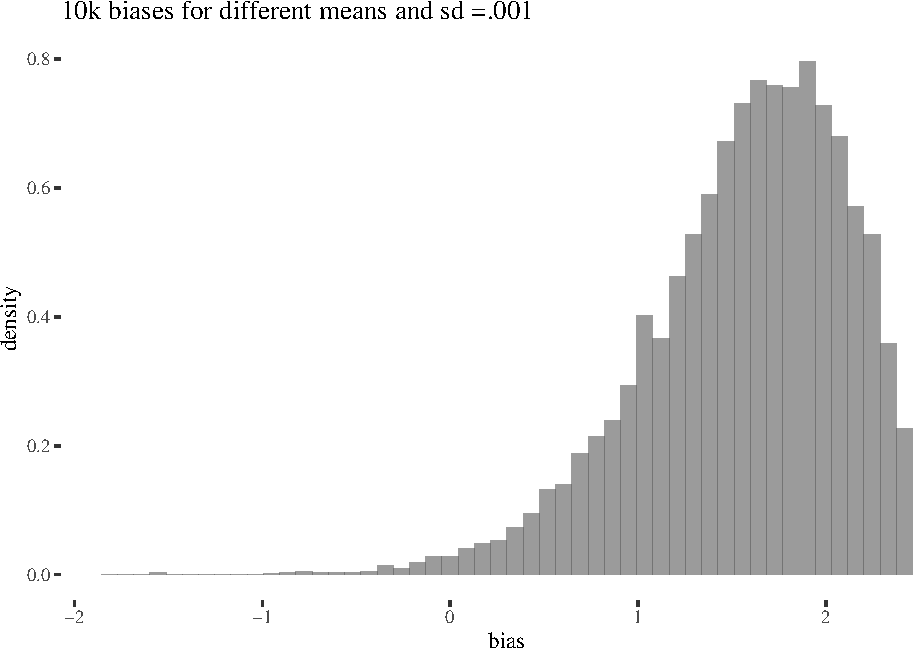
\includegraphics[width=1\linewidth]{paperDraft_files/figure-latex/unnamed-chunk-16-1} \end{center}

\normalsize

This is is a bit better, but still quite some uncertainty is involved,
far from what systematically low mean-based p-values reported in the
papers might suggest. Of course, this is a bit of a caricature, as our
word lists were short (four protected words and 10 attributes). But the
word lists used in the actually papers are not much longer. In such a
set-up the key observations are as follows:

\begin{itemize}
\item
  Seemingly high bias measures might arise even if the underlying
  processes actually have the same mean.
\item
  Even if the mean remains the same, non-negligible changes can result
  from a shift in the standard deviation of the original process, and
  the change might go in the opposite direction than a visualisation of
  datapoints might suggest, because with the decrease of standard
  deviation, the factor decreases and the bias increases.
\item
  Even if the underlying means are the same, but the variation is
  different, the bias metric in the long run could tend toward a
  different value:
\item
  The lack of control group in the paper and our analysis indicates that
  without neutral baseline it is difficult to interpret the
  effectiveness of the metric.
\end{itemize}

\vspace{1mm} \footnotesize

\begin{Shaded}
\begin{Highlighting}[]
\KeywordTok{mean}\NormalTok{(biasesD1); }\KeywordTok{mean}\NormalTok{(biasesD2)}
\end{Highlighting}
\end{Shaded}

\begin{verbatim}
## [1] 1.563319
\end{verbatim}

\begin{verbatim}
## [1] 1.690664
\end{verbatim}

\begin{Shaded}
\begin{Highlighting}[]
\KeywordTok{median}\NormalTok{(biasesD1); }\KeywordTok{median}\NormalTok{(biasesD2)}
\end{Highlighting}
\end{Shaded}

\begin{verbatim}
## [1] 1.638136
\end{verbatim}

\begin{verbatim}
## [1] 1.707511
\end{verbatim}

\normalsize
and so the point estimations of bias are sensitive to factors other than
the underlying process means.

\begin{itemize}
\item
  Even if there is a difference in means, the bias metric can be lower,
  and the uncertainty about it needs to be gauged.
\item
  The uncertainty resulting from including the raw datapoint variance
  into considerations is more extensive than the one suggested by the
  low p-values obtained from taking means as datapoints.
\end{itemize}

\vspace{1mm} \footnotesize

\begin{Shaded}
\begin{Highlighting}[]
\KeywordTok{quantile}\NormalTok{(biasesD2, }\DataTypeTok{probs =} \KeywordTok{c}\NormalTok{(}\FloatTok{0.275}\NormalTok{,}\FloatTok{0.975}\NormalTok{))}
\end{Highlighting}
\end{Shaded}

\begin{verbatim}
##    27.5%    97.5% 
## 1.539149 2.166488
\end{verbatim}

\begin{Shaded}
\begin{Highlighting}[]
\KeywordTok{quantile}\NormalTok{(biasesD1, }\DataTypeTok{probs =} \KeywordTok{c}\NormalTok{(}\FloatTok{0.275}\NormalTok{,}\FloatTok{0.975}\NormalTok{))}
\end{Highlighting}
\end{Shaded}

\begin{verbatim}
##    27.5%    97.5% 
## 1.300648 2.356815
\end{verbatim}

\normalsize

\section{Bayesian estimation}\label{bayesian-estimation}

We noticed that in Manzini et al. (2019) words from all three
sub-classes (in the case of religion by sub-class we mean Christianity,
Judaism, Islam) were compared against all of the stereotypes, which
means that there was no distinction between cases in which the
stereotype is associated with a given sub-class, as opposed to the
situation in which it is associated with another one. Not all of the
stereotypical words have to be considered as harmful for all of the
sub-groups. One should investigate the sub-groups separately as some of
them may have stronger harmful associations than others.

We decided to add control groups in the form of two classes --- neutral
words and human-related words. Without a proper control group it is
quite hard to compare the resulting cosine distances and decide on their
significance in bias detection. We prepared approximately 230 neutral
words to double-check the prima-facie neutral hypothesis that their
cosine similarity to the protected words will oscillate around 0 (that
is, the distances will be around 1). This provides us with a more
reliable point of reference. Moreover, we added human attributes that
are associated with people in general to investigate whether the smaller
cosine distance between protected words and stereotypes can result
simply from the fact that the stereotype predicates are associated with
humans.

One may consider improving the bias detection method presented in
Manzini et al. (2019). As the chosen protected words and attributes do
not represent the whole biased population but only a sample, it is
justified to introduce the uncertainty measure to the method. We decided
to use Bayesian estimation to make the cosine distance method more
methodologically correct.

Our priors distributions for the Bayesian model reflect our knowledge
about the data. The distribution for mean distance (cosine distance) is
set to be between 0 and 2 with the mean equal to 1. We assume that most
of the cosine distances may be considered neutral and therefore their
similarity will be small. The distribution for prior for standard
deviation is mostly between 0 and 1 with mean around 0. Finally the
distribution for prior for coefficients is mostly between -1 and 1, with
mean around 0. One should remember that the cosine distance values have
range between 0 and 2 therefore the choice of the prior distributions
should reflect this constraint. As we want to verify as objectively as
possible the assumptions present in Manzini et al. (2019) we decided to
use fairly weak and slightly skeptical regularizing priors. The models
parameters will have a posterior distribution obtained using either
Hamiltionian Monte Carlo methods (STAN) available through the rethinking
package.

\begin{center}
\begin{figure}[!htb]\centering
   \begin{minipage}{0.55\textwidth}
  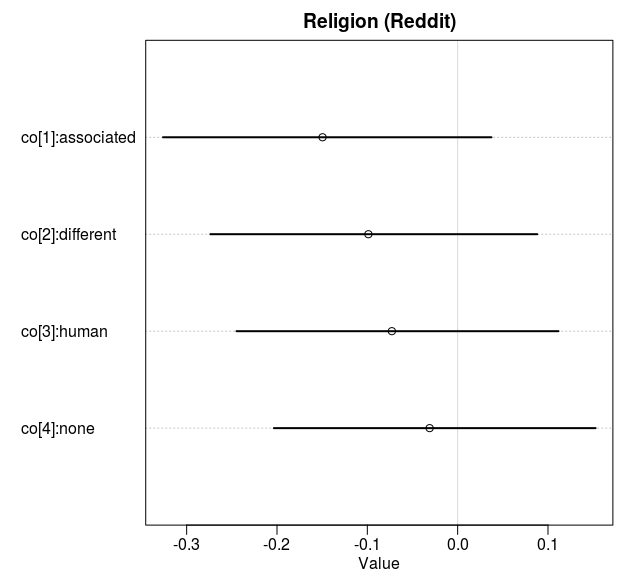
\includegraphics[width=7cm]{../images/religionCoeffs.jpeg}
   \end{minipage}
   \begin {minipage}{0.43\textwidth}
    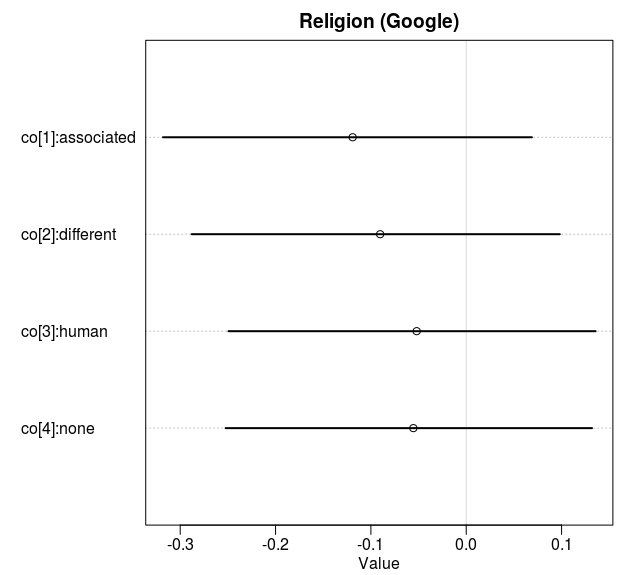
\includegraphics[width=7cm]{../images/religionGoogleCoeffs.jpeg}
   \end{minipage}
   
   
  \begin{minipage}{0.55\textwidth}
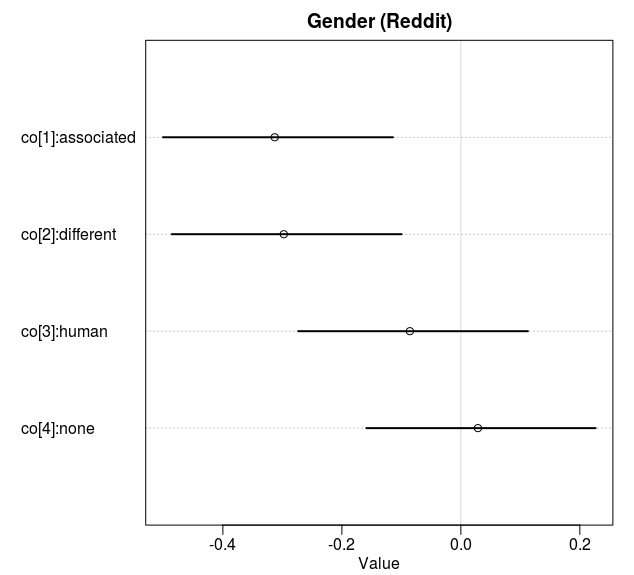
\includegraphics[width=7cm]{../images/genderCoeffs.jpeg}
\end{minipage}
   \begin {minipage}{0.43\textwidth}
    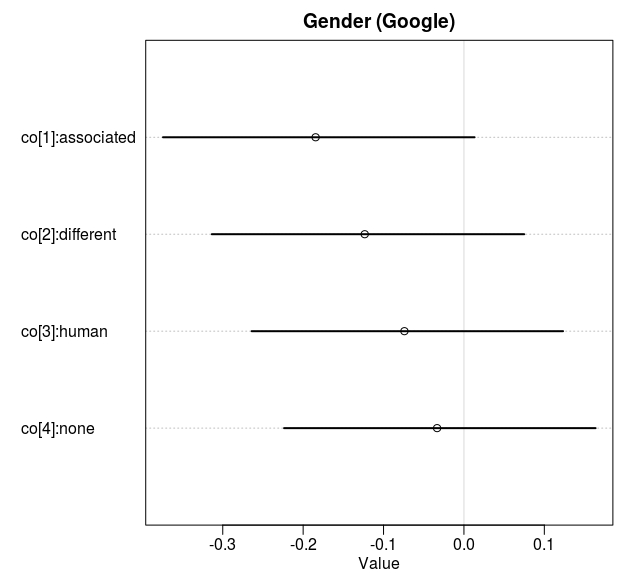
\includegraphics[width=7cm]{../images/genderGoogleCoeffs.jpeg}
   \end{minipage}
   
   
   
   
  \begin{minipage}{0.55\textwidth}
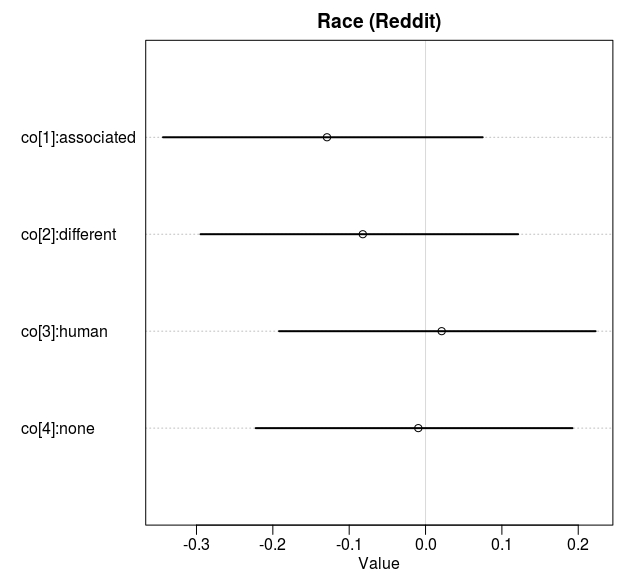
\includegraphics[width=7cm]{../images/raceCoeffs.jpeg}
\end{minipage}
   \begin {minipage}{0.43\textwidth}
    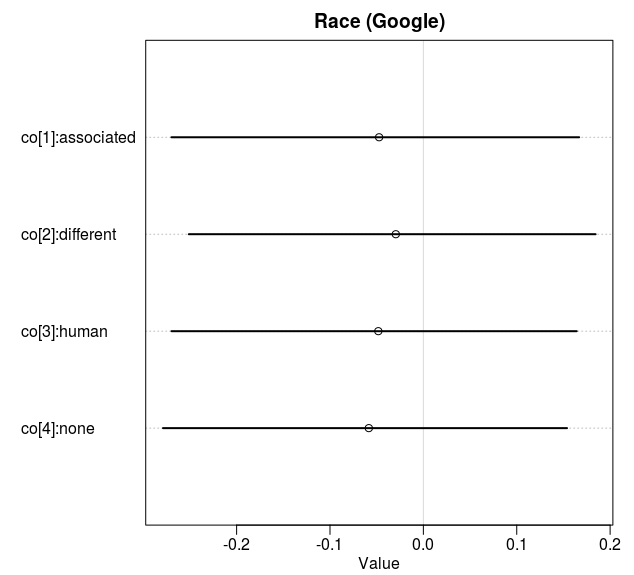
\includegraphics[width=7cm]{../images/raceGoogleCoeffs.jpeg}
   \end{minipage}
\end{figure}


\end{center}

Let's analyse dataset-level coefficients together with their highest
posterior density intervals, for the three topic groups. We compare the
results for two different word emebeddings corpuses - RedditL2 and
GoogleNews. For Google embeddings the HPDIs for all class coefficients
(associated, different, human, and none) include zero. This can lead one
to a conclusion that the impact for associated, different, human and
neutral attribute is, when averaged, quite similar. This indicates how
including the uncertainty may change the use and interpretation of
Manzini, Lim, Tsvetkov, \& Black (2019) MAC metric. It seems that if one
focuses only on differences between means of means, this is too
simplistic.

In the case of Reddit word embeddings the situation is similar although
HPDI is below 0 for Gender class when looking at \texttt{associated} and
\texttt{different} mean coefficient. This can suggest that there is
indeed slightly stronger impact of these attributes. One should also
notice how in general associated and different coefficients have quite
similar HPDI range, the highest observed absolute difference is equal to
only 0.1. This suggests that again the impact of associated attributes
and different ones is not clear at first sight. Finally, let's compare
the HPDIs for Reddit and Reddit debiased datasets. For Religion and Race
dataset there is a minor shift (in absolute values the highest change is
equal to approximately 0.1) of the mean coefficients towards zero.
However for Gender dataset there is no significant change. This is of
course a general look at the group coefficients. Let's now analyze the
individual words.

Looking at Reddit individual words one can observe that for Religion the
cosine distance results for the associated attributes are for most of
the words close to human attributes as well. This can suggest that in
some cases words concerning humans can have higher similarity with some
protected words independently of whether they are stereotypical or
neutral-human words. One should also pay attention to the fact that for
all of the associated and different attributes in Religion, the
uncertainty intervals overlap at some point. What is even more
surprising is that for protected words, such as ``torah'' the associated
attribute has the the cosine distance slightly over 1, which means no
positive similarity! If the protected words that we chose do not have
high similarity with harmful associated attributes, then one should
consider at least three scenarios. The first one is that the choice of
the protected words and attributes may be corrupted. The second one is
that the metric is unable to catch the hidden bias properly. The third
one is that there is actually no bias between the words. Regardless of
which scenario one considers, it is essential to take a look at the
individual values before averaging them or aggregating in other ways. It
seems that using Bayesian method can enhance the process of verifying
the hypotheses concerning the choice of protected words and attributes.

Surprisingly in Gender one can observe high cosine similarity values
between some female stereotypical professions and male protected words.
If a word stereotypically associated with females has low cosine
distance to male protected words, then one should investigate the issue
further. The reasons for this unexpected cosine distance may lie in the
frequency of appearance of the protected words in the raw data. Some of
the groups (like Muslim people or females) may have less representation
in the data that is taken as an input for word embeddings. Therefore, if
we assume that the MAC detects actually co-occurrence only, it makes
sense that they can have high similarity with associated attributes and
lower similarity with different ones. At the same time male protected
words and other religions can have high similarity with different
attributes because they have greater representation in the dataset in
general and occur close to much more concepts. Cosine distance seems to
capture the information on the co-occurrence of words and not on the
semantic similarity strictly speaking.

In Google, one may notice interesting phenomena as well. Although the
GoogleNews dataset is larger, trained on different data sources and with
the use of more dimensions, some of the results are similar to the ones
obtained for the Reddit corpus. For Religion almost all of the values
for associated class intersect with different class as well. In the case
of Race it is 100\% of the available words. This indicates again that it
is not clear how the metric should be used. Quite a different situation
takes place for Gender, where the similarity between associated and
different is present mostly for the male protected words. This means
that male words have high similarity with both male stereotypical
professions and female ones. However, for females, the similarity is
high mostly only for the female stereotypical professions. This
observation could not be made when using MAC metric only, as it requires
investigating the individual words, and providing uncertainty.

\section{Effects of debiasing}\label{effects-of-debiasing}

One may verify if the dataset-level coefficients changed after the
debiasing method used in Manzini et al. (2019). In some cases there is a
minor change to the right, the mean value is closer to 0. The
\texttt{associated} and \texttt{differen} attributes are now more
overlapping than before. However, the uncertainty intervals are still
high and therefore the significance of the change cannot be considered
as enormous. The surprising obervation is that in the case of
\texttt{Gender} and \texttt{Race} groups, the neutral words shifted to
the left, further from the neutral position.

\begin{center}
\begin{figure}[!htb]\centering
   \begin{minipage}{0.55\textwidth}
  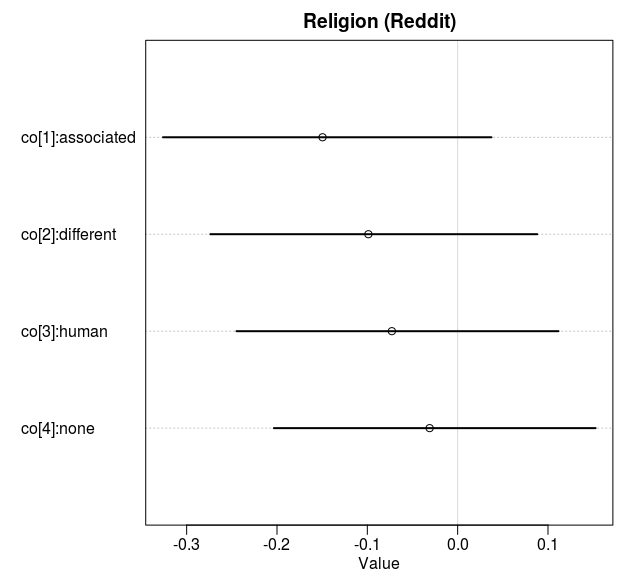
\includegraphics[width=7cm]{../images/religionCoeffs.jpeg}
   \end{minipage}
   \begin {minipage}{0.43\textwidth}
    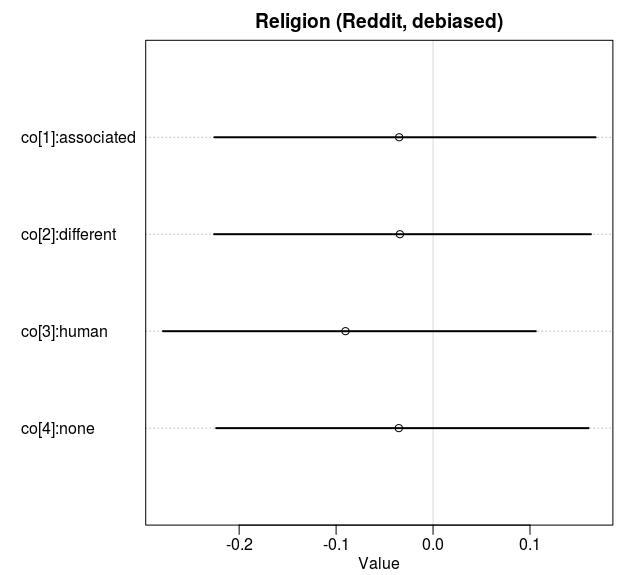
\includegraphics[width=7cm]{../images/debiasedReligionRedditCoeffs.jpeg}
   \end{minipage}
   
   
  \begin{minipage}{0.55\textwidth}
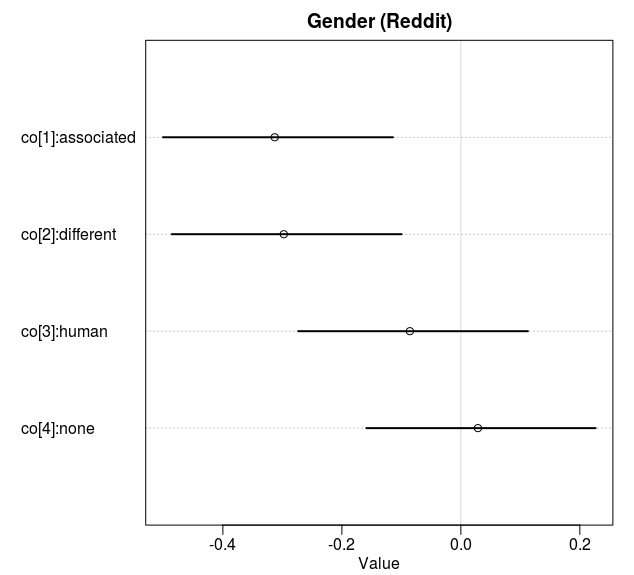
\includegraphics[width=7cm]{../images/genderCoeffs.jpeg}
\end{minipage}
   \begin {minipage}{0.43\textwidth}
    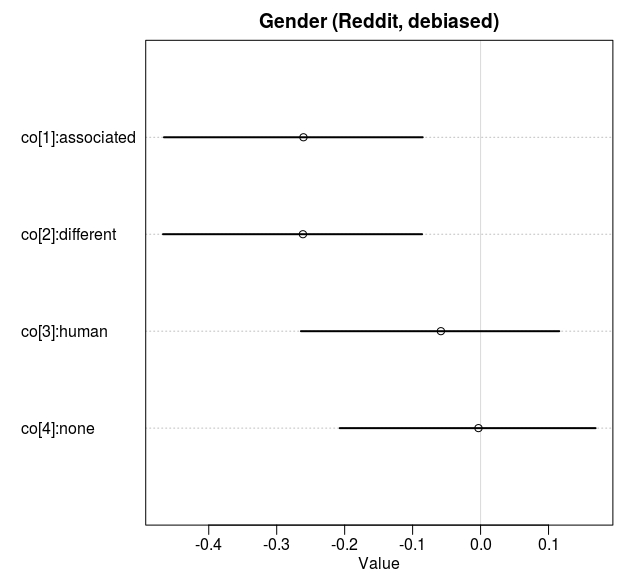
\includegraphics[width=7cm]{../images/debiasedGenderRedditCoeffs.jpeg}
   \end{minipage}
   
   
   
   
  \begin{minipage}{0.55\textwidth}
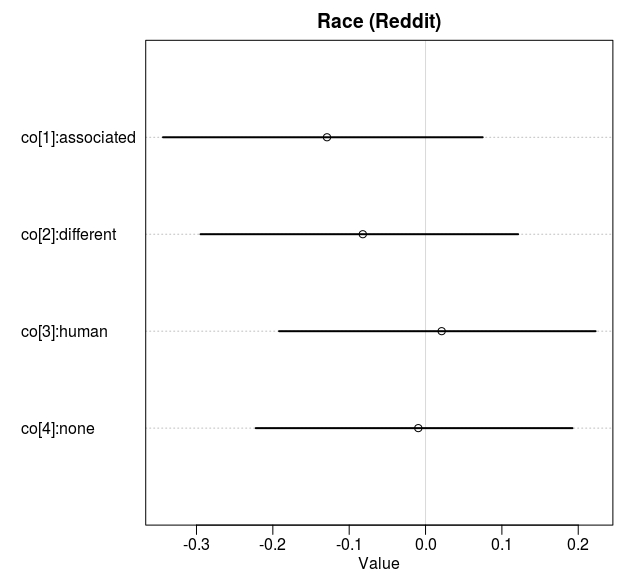
\includegraphics[width=7cm]{../images/raceCoeffs.jpeg}
\end{minipage}
   \begin {minipage}{0.43\textwidth}
    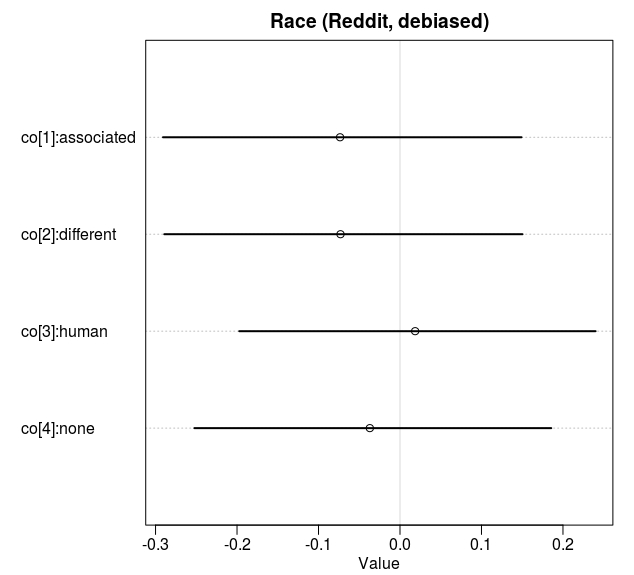
\includegraphics[width=7cm]{../images/debiasedRaceRedditCoeffs.jpeg}
   \end{minipage}
\end{figure}

\end{center}

When analyzing the Reddit debiased results one should investigate the
change of the individual cosine distance values as well. It seems that
not all of the protected words are treated equally when performing
debiasing. In religion, the values for associated class moved towards 0
for most of the words except for the ones for Islam, where still the
associated class has quite lower cosine distance than the different one.
Similar situation takes place in Gender, where female words have still
much lower cosine distance values for associated class than for the
different one. In the case of male protected words it is mostly almost
the same interval for associated and different. As the Gender data is
quite specific as the attributes are not harmful adjectives but (in an
ideal world) neutral professions, the aim (if we follow MAC assumptions)
should actually be to make the cosine distance same for both female and
male protected words. However, as we pointed out the situation after
debiasing can sometimes be better only for one protected group, which is
not the desired outcome. In the case of Religion, even after debiasing,
all of the protected words have intersections between associated and
different class and similarity greater than 0. As all of the attributes
in religion data are negative and harmful stereotypes, one should not
aim at making the distance between protected words and associated, and
different class the same but rather to move it towards 1.

\section{Discussion}\label{discussion}

\newpage

\noindent \huge  \textbf{Appendix} \normalsize

\noindent \Large \textbf{Word lists, including human and neutral predicates}
\normalsize

\section*{References}\label{references}
\addcontentsline{toc}{section}{References}

\vspace{-3mm}

\hypertarget{refs}{}
\hypertarget{ref-Manzini2019blackToCriminal}{}
Manzini, T., Lim, Y. C., Tsvetkov, Y., \& Black, A. W. (2019).
\emph{Black is to criminal as caucasian is to police: Detecting and
removing multiclass bias in word embeddings}.

\hypertarget{ref-Venkat2018Curse}{}
Venkat, N. (2018). \emph{The curse of dimensionality: Inside out}.
\url{https://doi.org/10.13140/RG.2.2.29631.36006}

\end{document}
